\documentclass[a4paper,12pt,oneside]{article}

\usepackage[utf8]{inputenc}
\usepackage[T2A]{fontenc}
\usepackage[russian]{babel}
\usepackage[usenames]{xcolor}
\usepackage{etoolbox}
\usepackage{listings}
\usepackage{graphicx}
\usepackage{cmap}
\usepackage{indentfirst}
\usepackage{makeidx}
\usepackage[unicode]{hyperref}

\newif\ifanswers
\answerstrue

\hypersetup{
%bookmarks=true,            % show bookmarks bar?
%unicode=false,             % non-Latin characters in Acrobat’s bookmarks
pdfproducer={Producer},    % producer of the document
pdfkeywords={keywords},    % list of keywords
pdfnewwindow=true,         % links in new window
colorlinks=true,           % false: boxed links; true: colored links
linkcolor=black,           % color of internal links
citecolor=black,           % color of links to bibliography
    filecolor=black,           % color of file links
    urlcolor=black             % color of external links
}

\renewcommand{\rmdefault}{cmr} 

\renewcommand{\texttt}[2][black]{\textcolor{#1}{\ttfamily #2}}

\renewcommand\floatpagefraction{0.8} %% default value: 0.5
\renewcommand\topfraction{0.8}       %% default value: 0.7

\definecolor{OliveGreen}{cmyk}{0.64,0,0.95,0.40}
\definecolor{mauve}{rgb}{0.58,0,0.82}

\setlength{\parskip}{6pt}

\makeindex

\title{Лекция по Toolchain}
\author{
  Владимиров Константин Игоревич\\
  \texttt{konstantin.vladimirov@gmail.com}
}
\date{\today}

\lstset{
language=C++,                           % Code langugage
basicstyle=\ttfamily,                   % Code font, Examples: \footnotesize, \ttfamily
keywordstyle=\color{OliveGreen},        % Keywords font ('*' = uppercase)
commentstyle=\color{gray},              % Comments font
stringstyle=\color{mauve},
numbers=left,                           % Line nums position
numberstyle=\tiny,
numbersep=10pt,
stepnumber=1,                           % Step between two line-numbers
frame=none,                             % A frame around the code
tabsize=2,                              % Default tab size
captionpos=b,                           % Caption-position = bottom
breaklines=true,                        % Automatic line breaking?
breakatwhitespace=false,                % Automatic breaks only at whitespace?
showspaces=false,                       % Dont make spaces visible
showstringspaces=false,
showtabs=false,                         % Dont make tabls visible
columns=flexible,                       % Column format
title=\lstname,
caption={},
extendedchars=\true,
inputencoding=utf8,
}

\begin{document}

\begin{titlepage}
\begin{center}

\large ~ \\[4.5cm]

\huge Конспект лекций\\[0.6cm]
\large По средствам разработки\\[3.7cm]

\begin{minipage}{0.5\textwidth} % начало маленькой врезки в половину ширины текста
\begin{flushleft} % выровнять её содержимое по левому краю
\emph{Автор:} Владимиров К. И.\\
\end{flushleft} % конец выравнивания по левому краю
\end{minipage} % конец врезки

\vfill

Страница с последней редакцией: \url{sourceforge.net/p/cpp-lects-rus}\\
Email автора: \texttt{konstantin.vladimirov@gmail.com}\\
{\large \today}
{\large \LaTeX}

\end{center}
\thispagestyle{empty}
\end{titlepage}

\tableofcontents

\pagebreak
\section{Toolchain}\label{sec:Toolchain}

Общеупотребительным англицизмом toolchain (можно перевести как ``набор средств разработки'' или как ``система компиляции'', можно оставить просто слово ``тулчейн'') обозначают набор средств разработки, совместно используемых для создания программного обеспечения. Обычно это компилятор, ассемблер, линкер, а также набор бинарных утилит. Иногда в состав toolchain включают средства отладки и верификации программ, профилировщики и анализаторы покрытия кода.

\subsection{Обзор средств разработки}\label{subsec:Overview}

Обычно весь набор средств разработки скрыт от пользователя за единой программой-драйвером (как в случае GNU Toolchain когда роль такой программы играет GCC) или за ширмой средств IDE (как в случае Microsoft Toolchain, когда компиляция ассемблирование и сборка происходят по нажатию кнопки F7 в Visual Studio).

Кроме GNU и Microsoft, известны также LLVM toolchain, Intel toolchain, ARM toolchain а также пакеты средств разработки Borland и Comeau. Для всех примеров ниже будет использоваться GNU Toolchain, но иногда будут приводиться примеры из других средств разработки, там, где есть некие концептуальные отличия. Точно также ниже будут описаны в основном примеры компиляции программ на языке C, разве что с некоторыми экскурсиями в C++ и Fortran.

Эта лекция ставит перед собой следующие цели:

\begin{itemize}
\item Сделать ясной структуру и последовательность работы системы компиляции в целом
\item Осветить роль каждого из инструментов в отдельности, его применимость и решаемые им задачи
\item Дать базу для самостоятельных экспериментов (на примере GNU Toolchain)
\item Изложить основные этапы портирования toolchain на новую архитектуру
\end{itemize}

Первый пункт можно переформулировать как простой и конкретный вопрос: что происходит при исполнении следующей строчки?

\begin{verbatim}
$ gcc program.c
\end{verbatim}

Правильный ответ: происходит запуск трёх основных программ, как это показано на (рис. \ref{fig:simplified_scheme}).

\begin{figure}[ht]
\centering
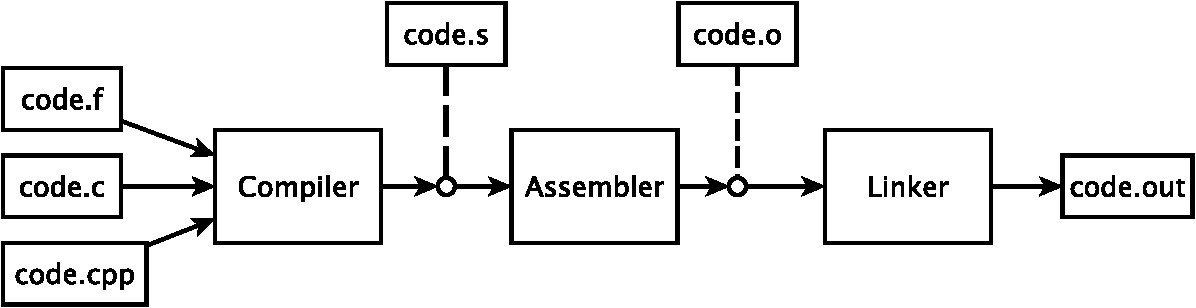
\includegraphics[width=1.0\textwidth]{illustrations/simplified-scheme-crop.pdf}
\caption{Упрощенная схема toolchain}
\label{fig:simplified_scheme}
\end{figure}

\begin{enumerate}
\item \textbf{Компилятор} -- в случае GNU toolchain это cc1 или cc1plus для кода на C или C++, в случае MSVS это cl.exe. Переводит текст на языке высокого уровня в язык ассемблера целевой архитектуры
\item \textbf{Ассемблер} -- в случае GNU toolchain это as, в случае MSVS это ml.exe. Кодирует ассемблер целевой архитектуры и порождает объектный код
\item \textbf{Линкер} -- в случае GNU toolchain это ld или gold, в случае MSVS это link.exe. Собирает несколько объектных модулей в исполняемый файл
\end{enumerate}

Toolchain не исчерпывается этой упрощенной схемой, но для начала рассмотрение трёх основных компонент позволяет создать общую картину происходящего.

\pagebreak
\subsection{Компилятор}\label{subsec:Compiler}

Компилятор является главным и наиболее известным компонентом средств разработки (автору не раз доводилось слышать как ``компилятором'' называют и драйвер и весь toolchain). Тем не менее, происходящее внутри компилятора часто также остается неизвестным разработчику, как и происходящее внутри системы компиляции в целом.

\begin{figure}[ht]
\centering
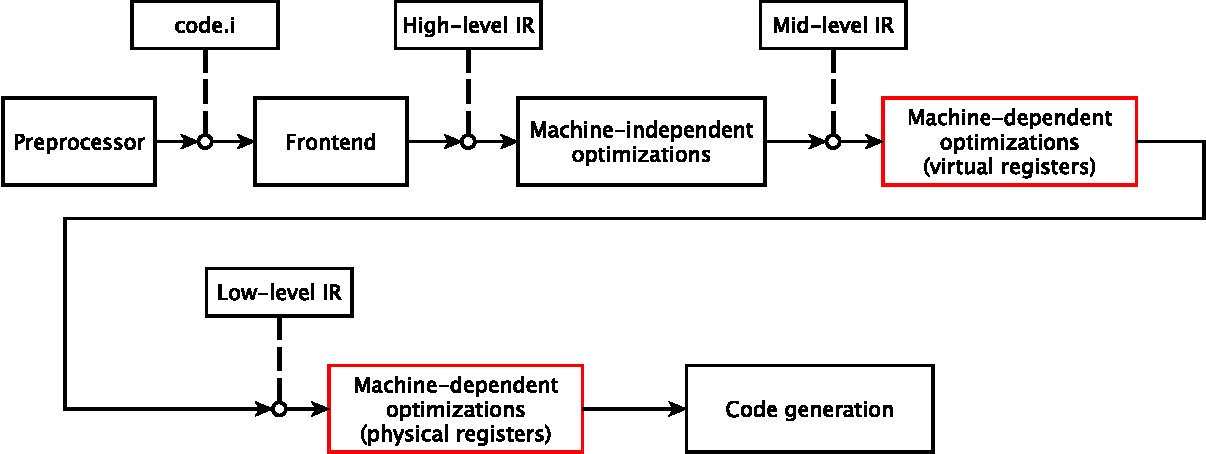
\includegraphics[width=1.0\textwidth]{illustrations/compiler-crop.pdf}
\caption{Компилятор изнутри}
\label{fig:compiler_scheme}
\end{figure}

На (рис. \ref{fig:compiler_scheme}) изображена схема работы компилятора, состоящая из следующих элементов:

\begin{enumerate}
\item \textbf{Препроцессор} -- занимается текстовой обработкой исходного текста и подготовкой к компиляции
\item \textbf{Фронтенд} -- переводит язык высокого уровня в промежуточное представление
\item \textbf{Бэкенд} -- состоит из оптимизаций на разных уровнях промежуточного представления и кодогенерации в ассемблер целевой архитектуры. Иногда его делят на middle-end, где выполняются машинно-независимые оптимизации и backend (выделен красным цветом), где происходят машинно-зависимые преобразования.
\end{enumerate}

В LLVM toolchain, препроцессор и фронтенд языков C и C++ вынесены в отдельную программу (clang), которая порождает машинно-независимое промежуточное представление (intermediate representation, или для краткости IR) над которым оптимизатор (подключаемый к clang как библиотека) производит преобразования до ассемблера. 

Препроцессор часто поставляется отдельно в наборе бинарных утилит, например в составе GNU Toolchain программа, производящая препроцессинг называется \textbf{cpp}. Она, тем не менее, не запускается в нормальной циклограмме работы, так как препроцессор является частью компилятора \textbf{cc1}, а cpp это просто отдельно лежащий препроцессор, отпиленный для удобства.

При достаточной универсальности IR, бэкенд тоже может быть вынесен как отдельная программа, таков например бэкенд llc, производящий трансформации LLVM IR и кодогенерацию. И llc и clang подключают одну и ту же библиотеку для использования в качестве бэкенда. Таким образом все три основные части тулчейна могут быть как совмещены в один исполняемый файл, так и разнесены по отдельным запускам в любых комбинациях.

\subsubsection{Препроцессор}\label{subsec:Preprocessor}

Работа препроцессора происходит в основном над текстом и в случае языка C регламентирована стандартом языка (5.1.1.2 в C11). В случае gcc, для препроцессирования файла имеется опция -E.

\begin{figure}[ht]
\centering
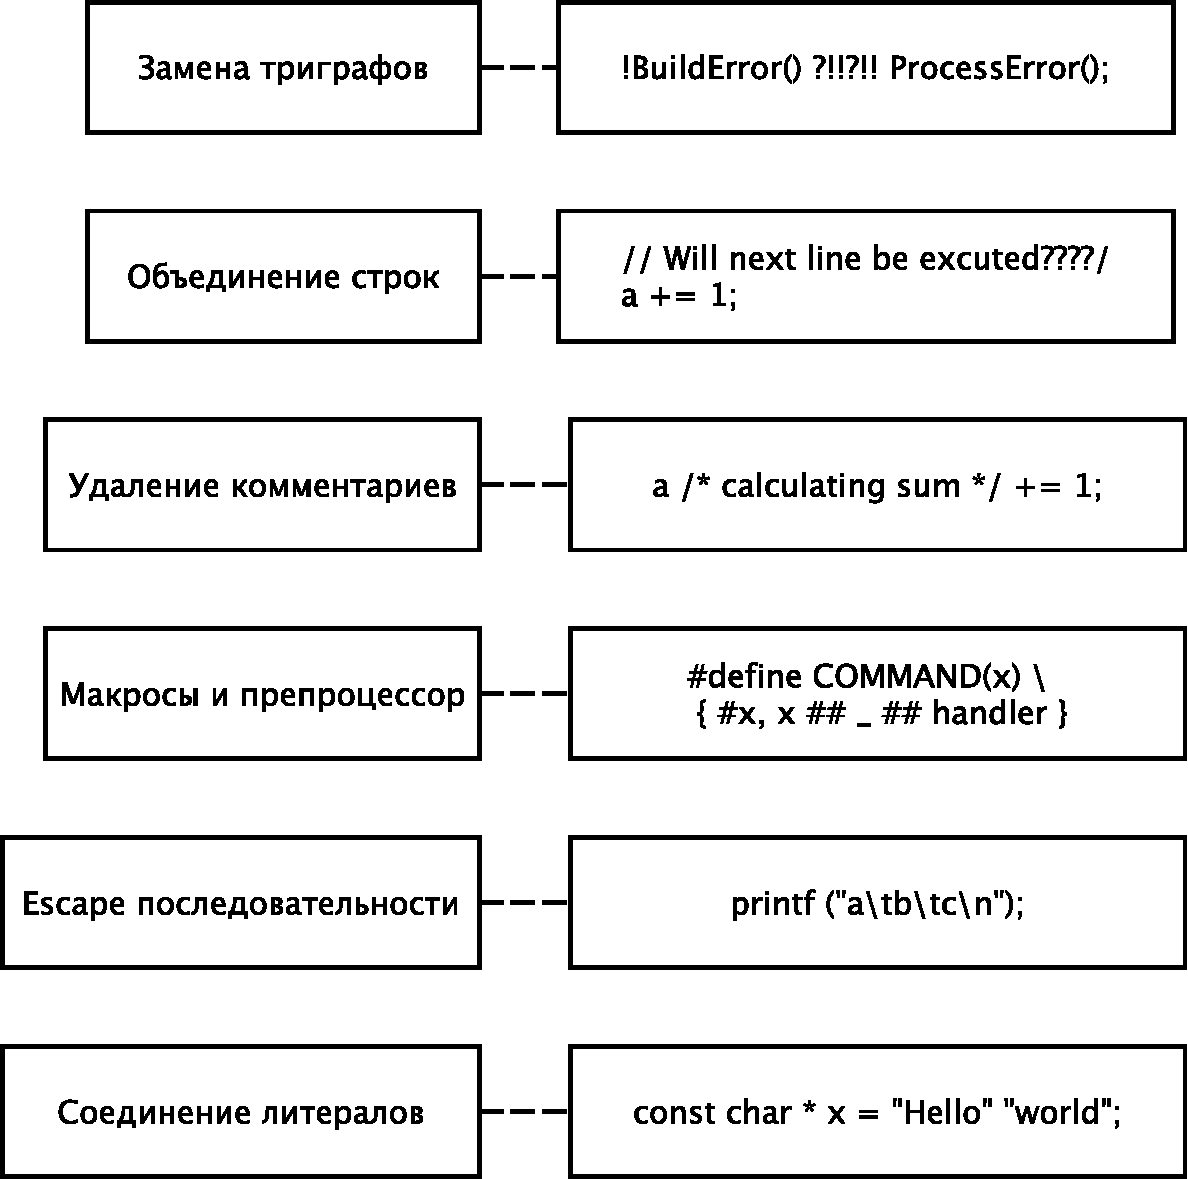
\includegraphics[width=0.8\textwidth]{illustrations/preprocessor-scheme-crop.pdf}
\caption{Схема препроцессора}
\label{fig:preproc_scheme}
\end{figure}

Препроцессор, как это изображено на (рис. \ref{fig:preproc_scheme}) выполняет действия в следующем порядке:

\begin{itemize}
% в 2017 году триграфы должны запретить, тогда этот пункт следует удалить, а остальные переписать
\item Замена триграфов 

Наиболее эзотерическая часть работы. Триграфы это специальные последовательности символов ориентированные на консоли где не было возможности ввести и обработать некоторые спецсимволы языка. Код с использованием триграфов выглядит действительно необычно. Например попробуйте понять что происходит на этой строчке: 

\begin{lstlisting}
!ErrorOccured() ??!??! HandleError();
\end{lstlisting}

Правильный ответ -- здесь вместо вертикальной черты использован триграф \lstinline$??!$ так что непонятная мешанина знаков в середине это просто длинное или. Ещё пример: 

\begin{lstlisting}
// WTF????/
a += 1;
\end{lstlisting}

Здесь использован триграф \lstinline$??/$, обозначающий обратный слеш. Что приводит к следующему пункту.

\item Объединение строк по обратному слешу

В примере выше после раскрытия триграфа остаётся:
\begin{lstlisting}
// WTF??\
a += 1;
\end{lstlisting}
И на этом этапе эти строки будут объединены в:
\begin{lstlisting}
// WTF??a += 1;
\end{lstlisting}

\item Разбиение на токены препроцессирования и замена комментариев пробелами

Здесь будут вычеркнуты все комментарии и заменены одним пробельным символом.

\item Раскрытие макросов и обработка директив препроцессора

На этом этапе раскрываются все макро-определения, как явно введенные через директиву \lstinline!#define! так и неявно заданные как билтины компилятора (скажем \lstinline!__cplusplus! позволяющий отличить компиляцию на C и C++). В случае GNU Toolchain, посмотреть встроенные макроопределения можно с помощью опций -E -dM.

\item Замена escape-последовательностей

Я полагаю, все встречались с escape-последовательностями \lstinline!\n! (перенос строки) или \lstinline!\t! (табуляция) при использовании функции printf и ей подобных. На самом деле их гораздо больше, например \lstinline!\0! можно использовать для обозначения завершающего нуля в строковом литерале. Полный список всегда можно посмотреть в стандарте языка.

\item Соединение стоящих рядом строковых литералов

Это позволяет писать строчки вида:

\begin{lstlisting}
#define HELLO "Hello"
printf (HELLO ", world!\n");
\end{lstlisting}

После макроподстановки, получившийся составной литерал \lstinline!"Hello" ", world\n"! пройдет конкатенацию строк и превратится в одну строку.
\end{itemize}

Файл, получившийся после препроцессирования, называется единицей трансляции (translation unit) и обрабатывается компилятором. В некоторых языках (например Fortran) несколько единиц трансляции могут располагаться в одном файле.

\subsubsection{Фронтенд}\label{subsubsec:Frontend}

Фронтенд компилятора работает с препроцессированным файлом и выполняет тяжелую задачу разбора языковых конструкций и перевода программы с конкретного языка программирования (например C++) в высокоуровневое промежуточное представление, удобное для машинно-независимых оптимизаций. Обычно фронтенд осуществляет:

\begin{itemize}
\item Лексический анализ: выделение ключевых слов языка, имён переменных и символов операций
Пример: \lstinline!int z = x+++y;! будет распознано как \lstinline!int z = (x++)+y;! (слева направо) но при этом \lstinline!int z = x = y;! будет распознано как \lstinline!int z = (x = y);! (справа налево)
\item Синтаксический анализ и построение дерева синтаксического разбора (см. пример на рис. \ref{fig:ast_scheme})
\item Анализ и вывод типов выражений
\end{itemize}

\begin{figure}[ht]
\centering
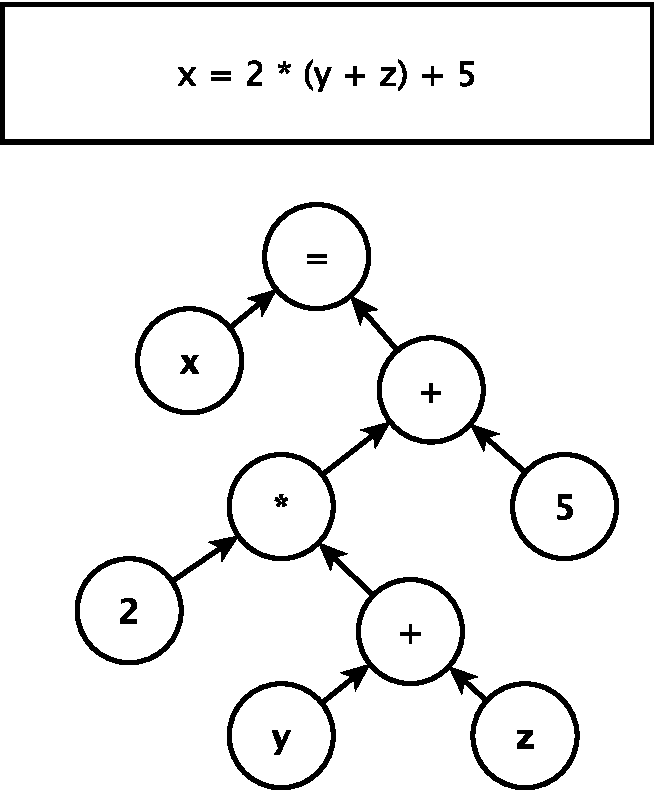
\includegraphics[width=0.5\textwidth]{illustrations/ast-example-crop.pdf}
\caption{Дерево синтаксического разбора}
\label{fig:ast_scheme}
\end{figure}

Иногда фронтенду приходится решать довольно сложные задачи связанные с тем, что современные языки высокого уровня (такие как C++) могут иметь неочевидный синтаксис и семантику.

Классический пример:

\begin{lstlisting}
ifstream datafile ("ins.dat");
list<int> data (istream_iterator<int>(dataFile),
                istream_iterator<int>());
\end{lstlisting}

Может показаться удивительным, но вторая строчка содержит объявление функции, а вовсе не заполнение контейнера из файла. Спасает простановка скобок:

\begin{lstlisting}
ifstream datafile ("ins.dat");
list<int> data ((istream_iterator<int>(dataFile)),
                istream_iterator<int>());
\end{lstlisting}

Ещё один пример:

\begin{lstlisting}
template <class T>
foo (T x)
{
  T::iterator *y;
  /* .... */
}
\end{lstlisting}

Увы, без дополнительных подсказок, синтаксический разбор определяет это как умножение некоего статического члена \lstinline!T::iterator! на некоторую глобальную переменную \lstinline!y!. Чтобы помочь фронтенду, здесь уместно добавить ключевое слово \lstinline!typename!:

\begin{lstlisting}
template <class T>
foo (T x)
{
  typename T::iterator *y;
  /* .... */
}
\end{lstlisting}

Как правило, результатом работы фронтенда является промежуточное представление (Gimple в случе GCC, LLVM IR в случае LLVM и так далее).

\subsubsection{SSA представление}\label{subsubsec:SSA}

SSA это аббревиатура для static single assignment. Программа считается представленной в SSA-форме, если каждой именованной переменной в программе может быть только один раз присвоено значение. Одним из важных следствий этого определения является referencial transparency -- то свойство программы, когда значение переменной независимо от её положения в программе.

\begin{lstlisting}
x = 1;
y = x + 1;
x = 2;
z = x + 1;
\end{lstlisting}

Эта программа является корректным кодом на C, но значение \lstinline!x! зависит от анализируемой строчки, в результате чего \lstinline!y = x + 1! и \lstinline!z = x + 1! имея идентичную форму определения, имеют разные значения. В случае SSA-формы этот код может быть переписан:

\begin{lstlisting}
x1 = 1;
y = x1 + 1;
x2 = 2;
z = x2 + 1;
\end{lstlisting}

Здесь очевидно, что разные значения соответствуют разной форме определения. Но для линейных участков всё просто. Сложнее преобразовать в SSA форму ветвления. Например:

\begin{lstlisting}
x = input ();
if (x > 42)
  y = 1;
else
  y = x - 2;
use (y);
\end{lstlisting}

Здесь для того, чтобы избавиться от двух определений \lstinline!y! нужно ввести $\phi$-функцию которая будет ``выбирать'' верное значение \lstinline!y! из двух пришедших к ней $y_1$ и $y_2$ как показано на рисунке:

\begin{figure}[h!]
\centering
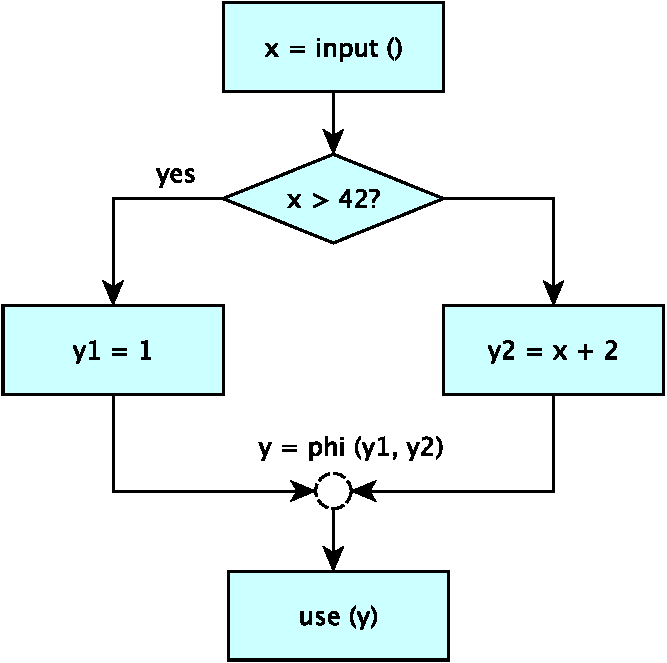
\includegraphics[width=0.6\textwidth]{illustrations/ssa-romb-crop.pdf}
\caption{$y = \phi(y_1, y_2)$}
\label{fig:ssa_romb_scheme}
\end{figure}

Изначально такие функции получили своё название от phony-functions (фальшивые функции), но название прижилось и сократилось. Обозначения \lstinline!phi(y1, y2)! и $\phi(y_1, y_2)$ далее будут достаточно свободно взаимозаменяемы.

К сожалению, их никак нельзя переписать на C, но в GIMPLE дампах они выглядят так:

\begin{lstlisting}
  <bb 3>:
  # n_5 = PHI <5(2), _6(4)>
  # mult_acc_7 = PHI <1(2), mult_acc_8(4)>
...
\end{lstlisting}

Эта запись означает, что есть два пути, по которым управление сходится в \lstinline!bb3! из блоков \lstinline!bb2! (там где в скобках стоит 2) и \lstinline!bb4! для \lstinline!n_5!, причём внутри \lstinline!bb2! определение этой переменной имеет имя \lstinline!5! (по правилам GIMPLE это просто константа 5), а в \lstinline!bb4! имеет имя \lstinline!_6! (искуственно созданные временные переменные в GIMPLE часто имеют безликие имена \lstinline!_1!, \lstinline!_2! и так далее).

\subsubsection{Машинно-независимые преобразования}\label{subsubsec:MITrans}

Для примера работы промежуточного представления можно рассмотреть функцию, вычисляющую (с первого взгляда -- крайне неоптимально) факториал числа, переданного в качестве аргумента.

\begin{lstlisting}
unsigned
fact (unsigned x)
{
  if (x < 2)
    return 1;

  return x * fact (x-1);
}
\end{lstlisting}

Трансформации сильно зависят от опций конкретного компилятора, рассмотрим этот пример как скомпилированный с \lstinline!-O2! в 64-битном режиме (обычно чем выше уровень, тем сильнее оптимизация, уровень 2 означает применять большинство полезных оптимизаций и оптимизировать код по скорости исполнения).

После работы фронтенда GCC, эта функция представлена в виде машинно-независимого языка промежуточного представления GIMPLE. В виде графа её можно изобразить как показано на рис. \ref{fig:fact_gimple_ssa}.

\begin{figure}[ht]
\centering
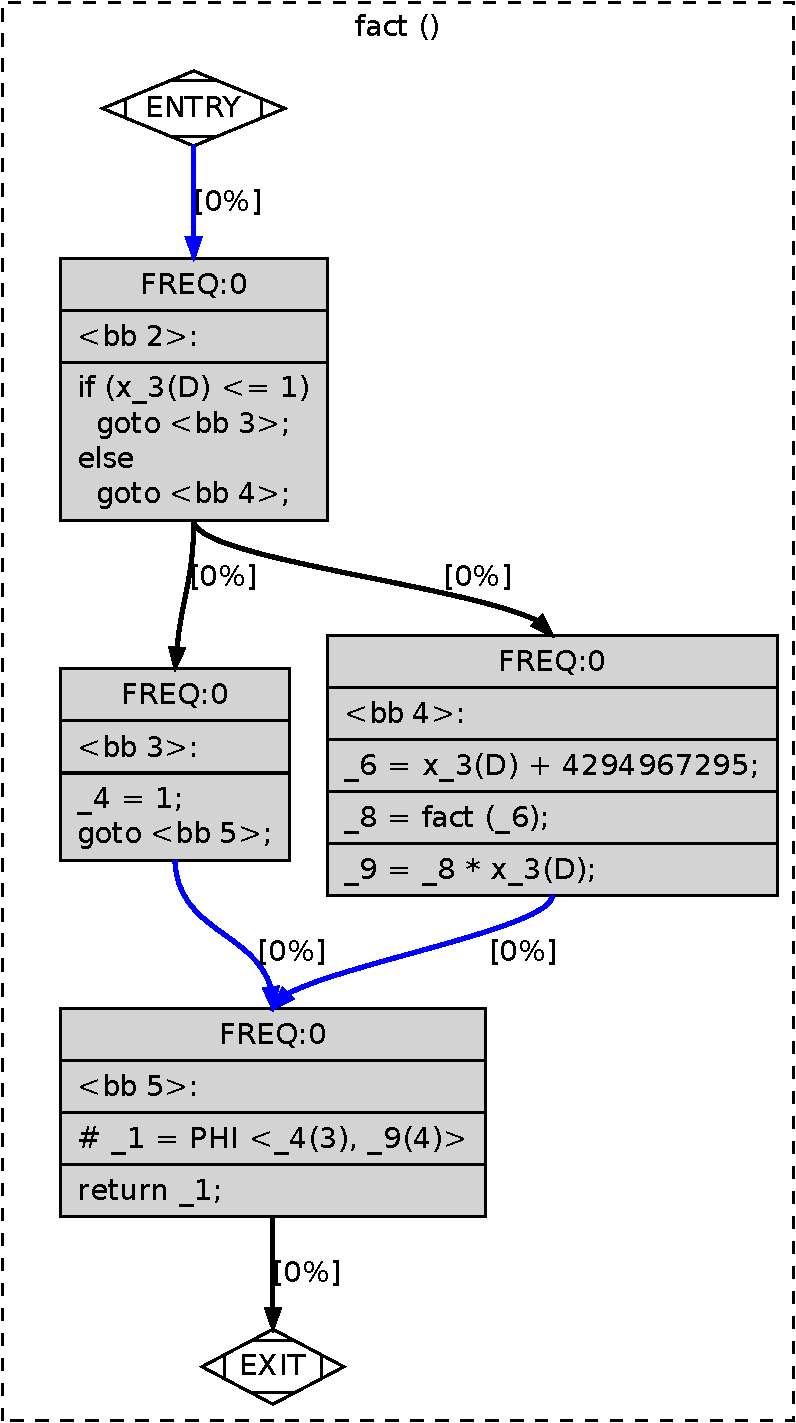
\includegraphics[width=0.5\textwidth]{illustrations/fact-ssa-crop.pdf}
\caption{GIMPLE на начальных фазах}
\label{fig:fact_gimple_ssa}
\end{figure}

Для получения дампа, можно воспользоваться опцией \lstinline!-fdump-tree-ssa! а в общем случае опцией \lstinline!-fdump-tree-all! позволит посмотреть все результаты работы всех фаз на уровне GIMPLE.

Программа на рис. \ref{fig:fact_gimple_ssa} практически повторяет структуру исходного кода на C, с учётом перевода в SSA и расстановки $\phi$-функций. Далее за дело берутся машинно-независимые оптимизации, которых в GCC 5.2 насчитывается более двухсот. Уже через несколько итераций происходит подстановка хвостового вызова и код начинает выглядет гораздо интереснее, как показано на (рис. \ref{fig:fact_gimple_release_ssa}).

\begin{figure}[ht]
\centering
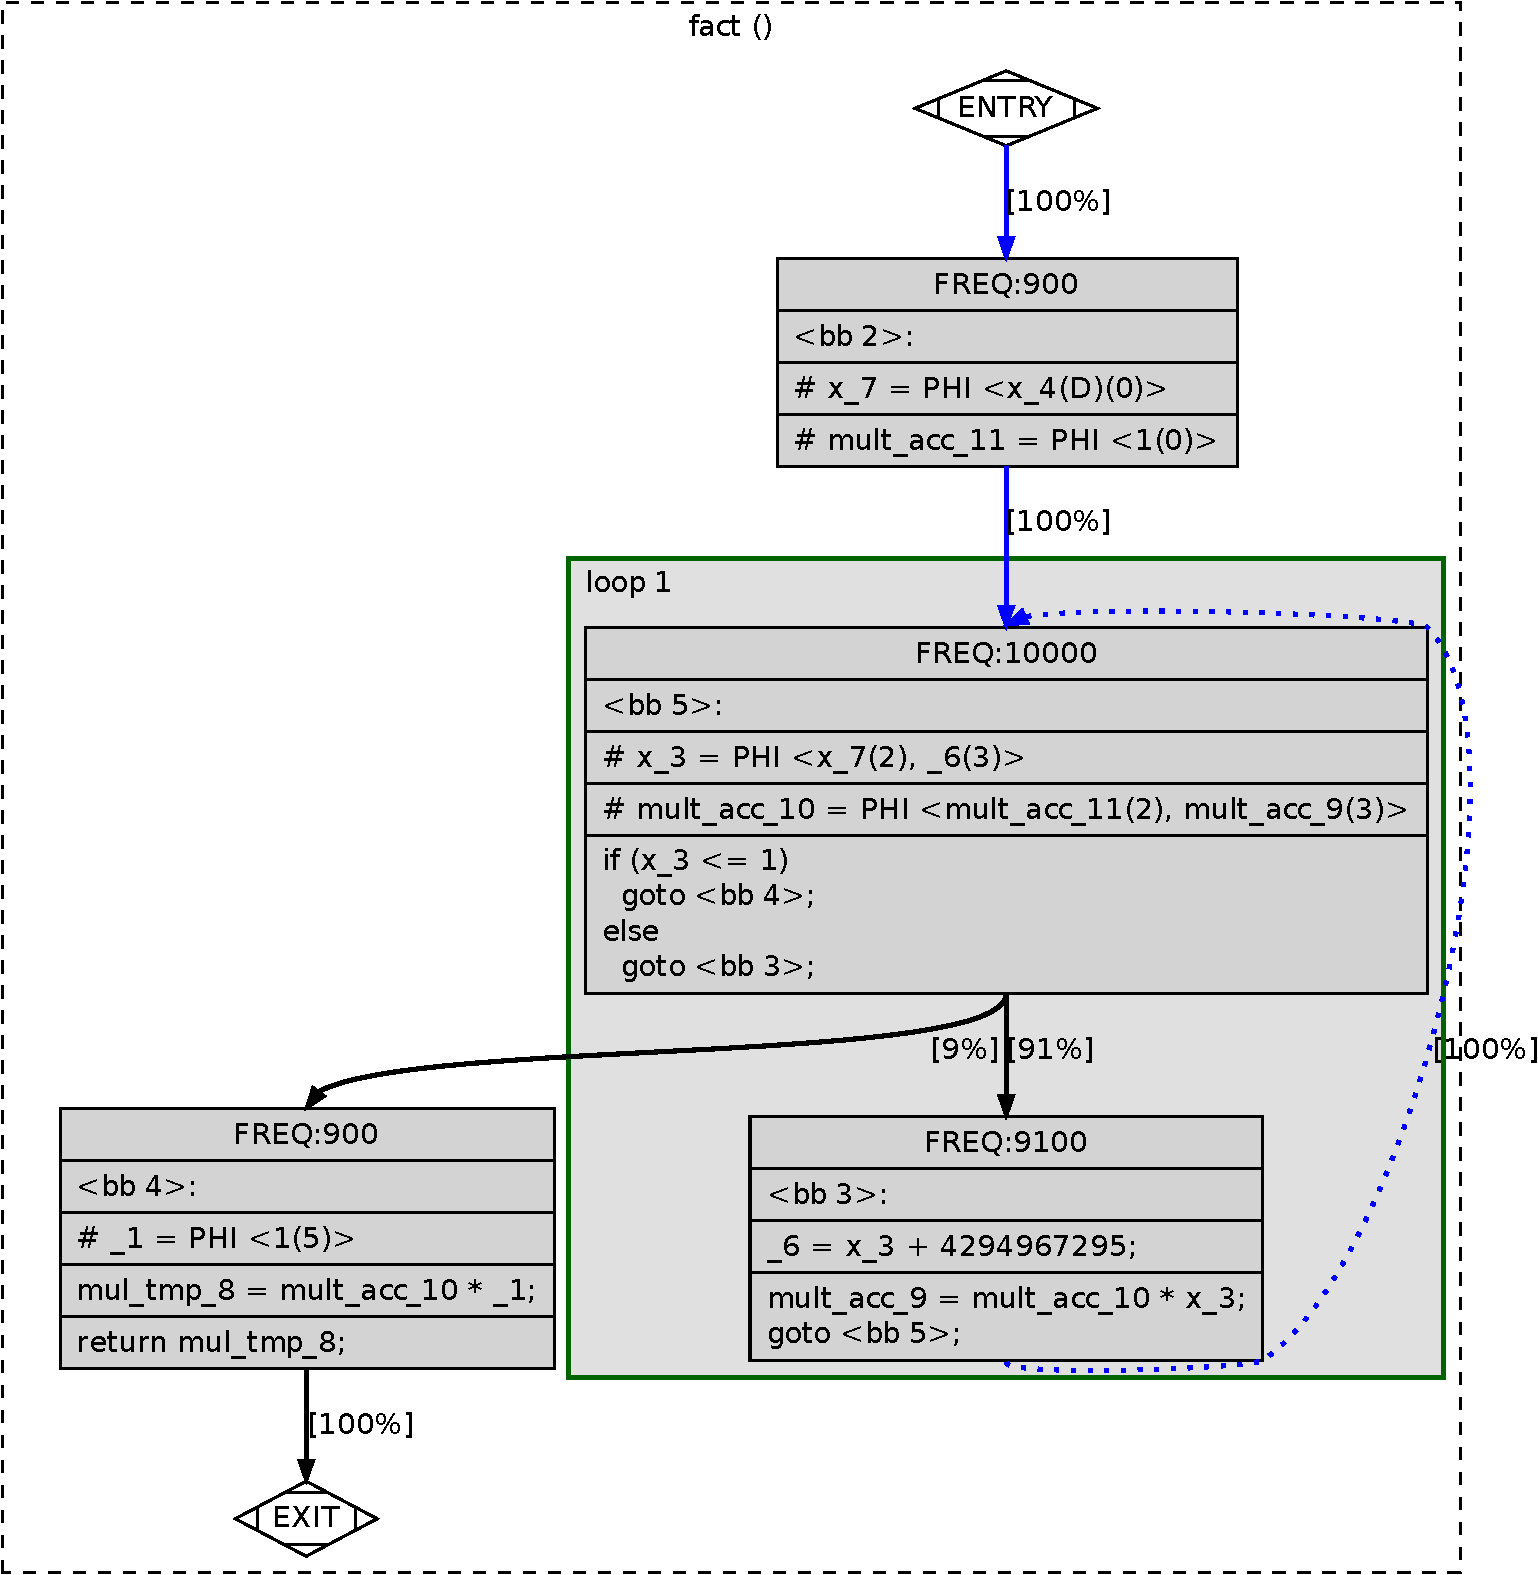
\includegraphics[width=0.9\textwidth]{illustrations/fact-release_ssa-crop.pdf}
\caption{GIMPLE после tail-call оптимизаций}
\label{fig:fact_gimple_release_ssa}
\end{figure}

Пунктирной линией показана обратная дуга цикла, который получился в результате раскрытия хвостовой рекурсии. Кроме того, следует обратить внимание на расставленные вероятности переходов -- здесь они расставлены компилятором априорно. Их можно сделать гораздо более точными если использовать при компиляции профиль реального запуска программы.

\subsubsection{Машинно-зависимые преобразования}\label{subsubsec:MDTrans}

После окончания машинно-независимых преобразований, код переводится в машинно-зависимую форму, называемую в случае GCC register transfer language или RTL. Интересно, что этот перевод называется по разному в разных компиляторах. В мире LLVM говорят ``lowering'' выражая этим понижение уровня представления. В мире GCC говорят ``expand'' -- раскрытие машинно-независимых конструкций в машинно-зависимый формат.

Все инструкции в машинно-зависимом формате зависят от описания конкретной машины в бэкенде компилятора и на ранних фазах RTL оперируют с виртуальными регистрами. Виртуальные регистры это не SSA представление, это абстрактная регистровая машина, в которой количество регистров не ограничено.

Получить дампы RTL в GCC можно с помощью опции \lstinline!-fdump-rtl-all!, где, как обычно, вместо all можно подать символическое имя фазы (\lstinline!-fdump-rtl-expand! для кода сразу после раскрытия и так далее).

Чтение дампов RTL осложняется тем фактом, что они представлены в сложном LISP-подобном формате:

\begin{verbatim}
(insn 15 14 16 5 (parallel [
            (set (reg:SI 90 [ D.1850 ])
                (mult:SI (reg:SI 90 [ D.1850 ])
                    (reg/v:SI 92 [ x ])))
            (clobber (reg:CC 17 flags))
        ]) -1
     (nil))
\end{verbatim}

На самом деле выше происходит следующее: в виртуальный регистр с номером 90 записывается произведение виртуальных регистров 90 и 92, параллельно с чем непредсказуемо изменяется флаговый регистр. Для простоты это можно записать как:

\begin{lstlisting}
v90 = v90 * v92;
clobber (v17);
\end{lstlisting}

Здесь буква v подчеркивает, что регистры виртуальные. На рис. \ref{fig:fact_rtl_expand} изображен код факториала сразу после раскрытия в машинно-зависимый формат.

\begin{figure}[htb]
\centering
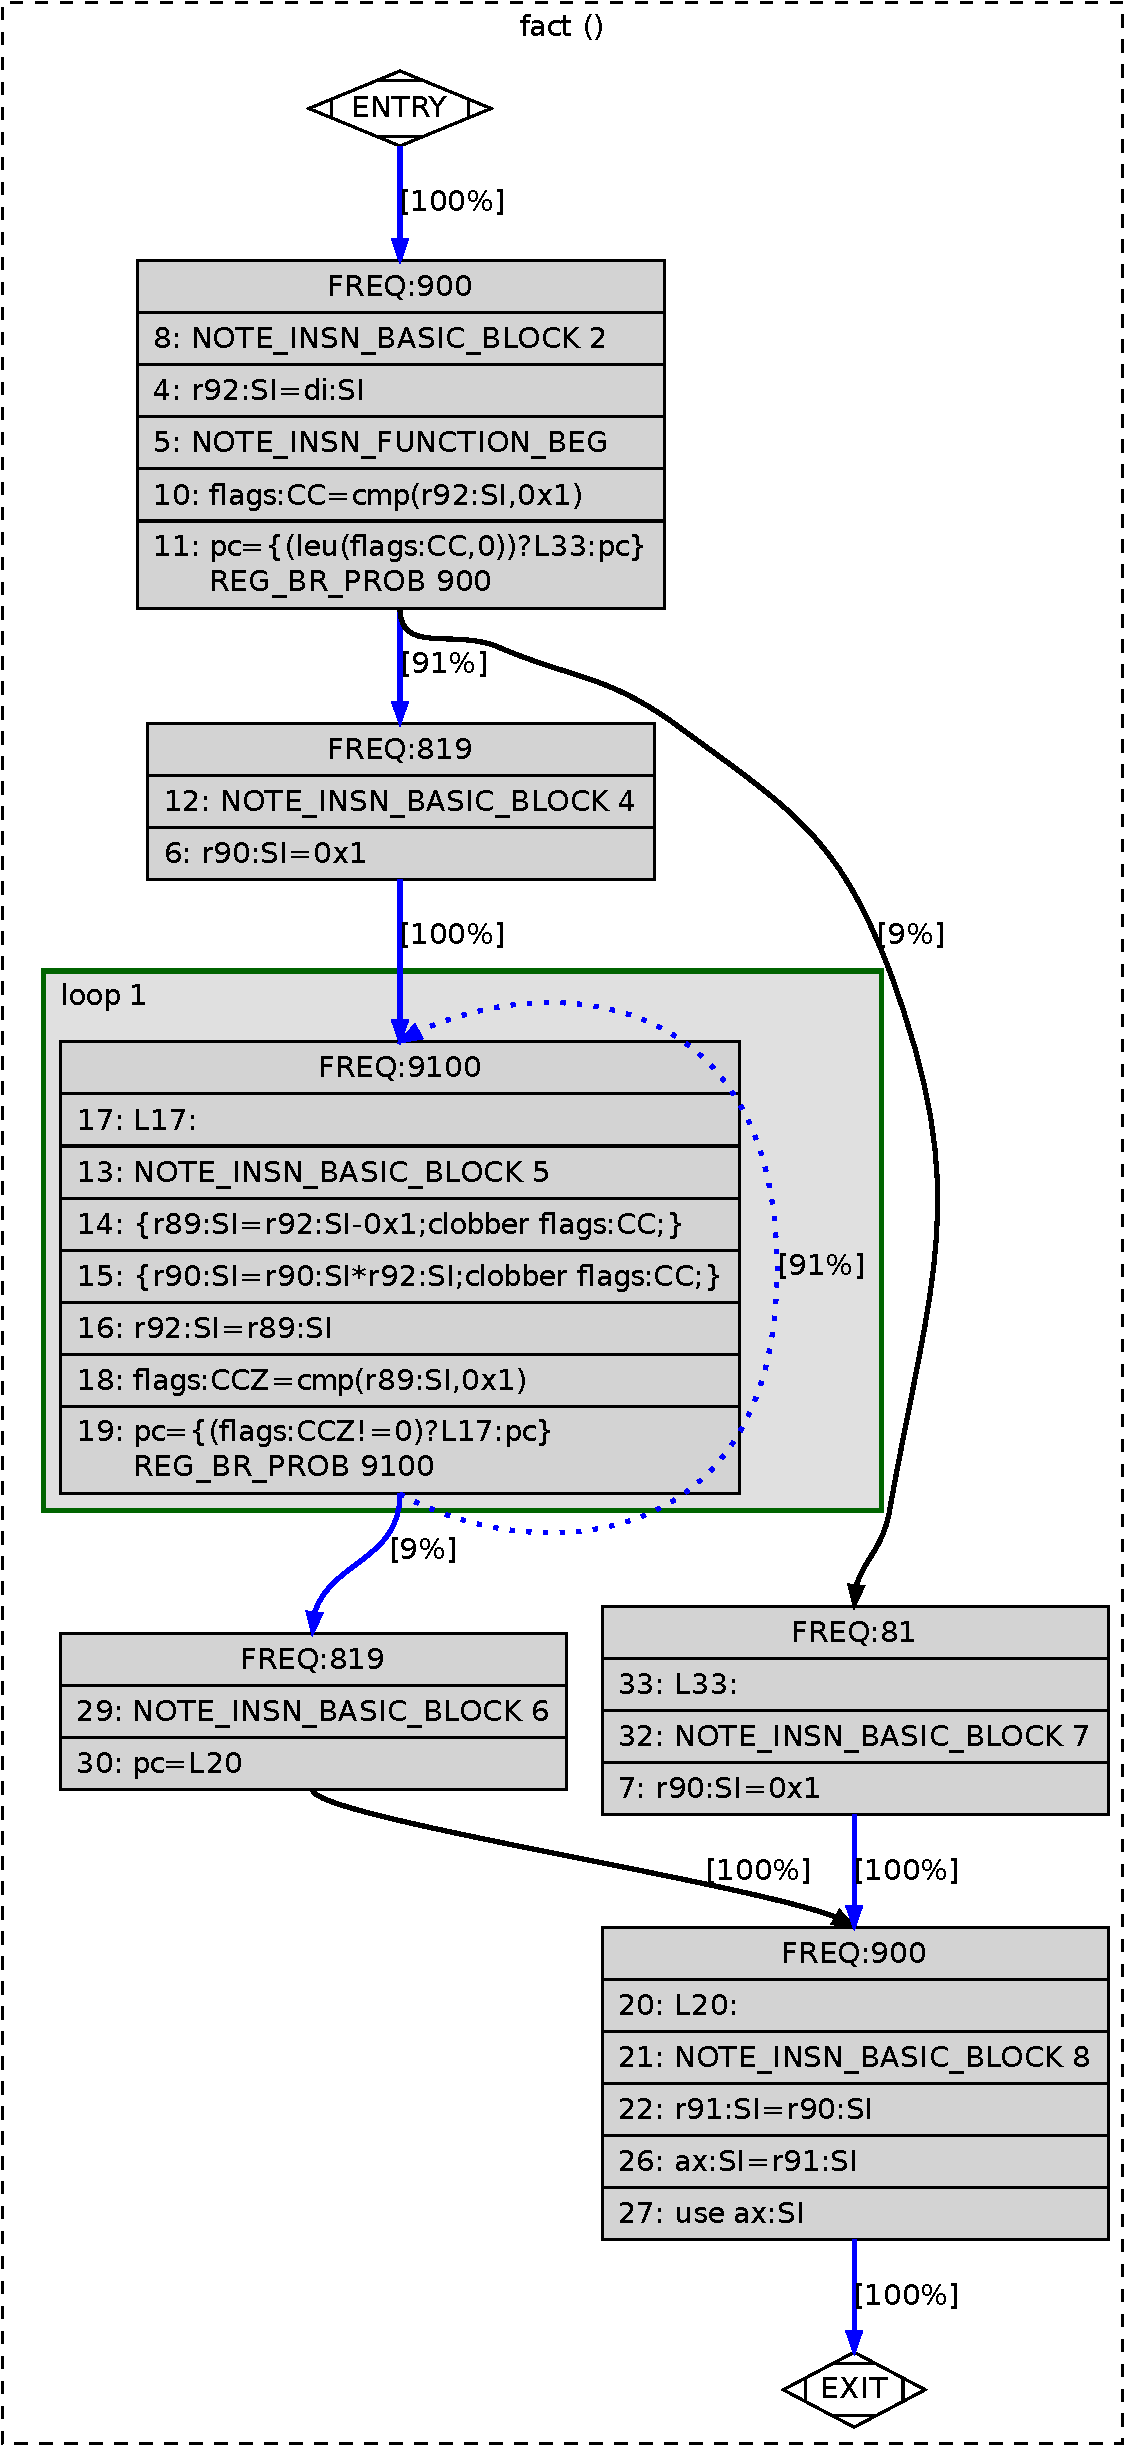
\includegraphics[height=0.7\textheight]{illustrations/fact-expanded-crop.pdf}
\caption{RTL с виртуальными регистрами}
\label{fig:fact_rtl_expand}
\end{figure}

Можно заметить, что каждому регистру сопоставлен режим (register mode) в котором он используется. Некоторые из этих режимов перечисленны ниже:

\begin{enumerate}
\item SI -- одно машинное слово (single integer mode). Обычно соответствует 32 битам.
\item DI, HI, QI -- двойное слово, половинное и четверть слова (double, half, quad)
\item CC, CCZ -- регистры флагов
\end{enumerate}

Использование виртуального регистра в каком-то режиме не отменяет того, что после окончания жизни этой переменной он не будет переиспользован в каком-то другом режиме.

\begin{figure}[htb]
\centering
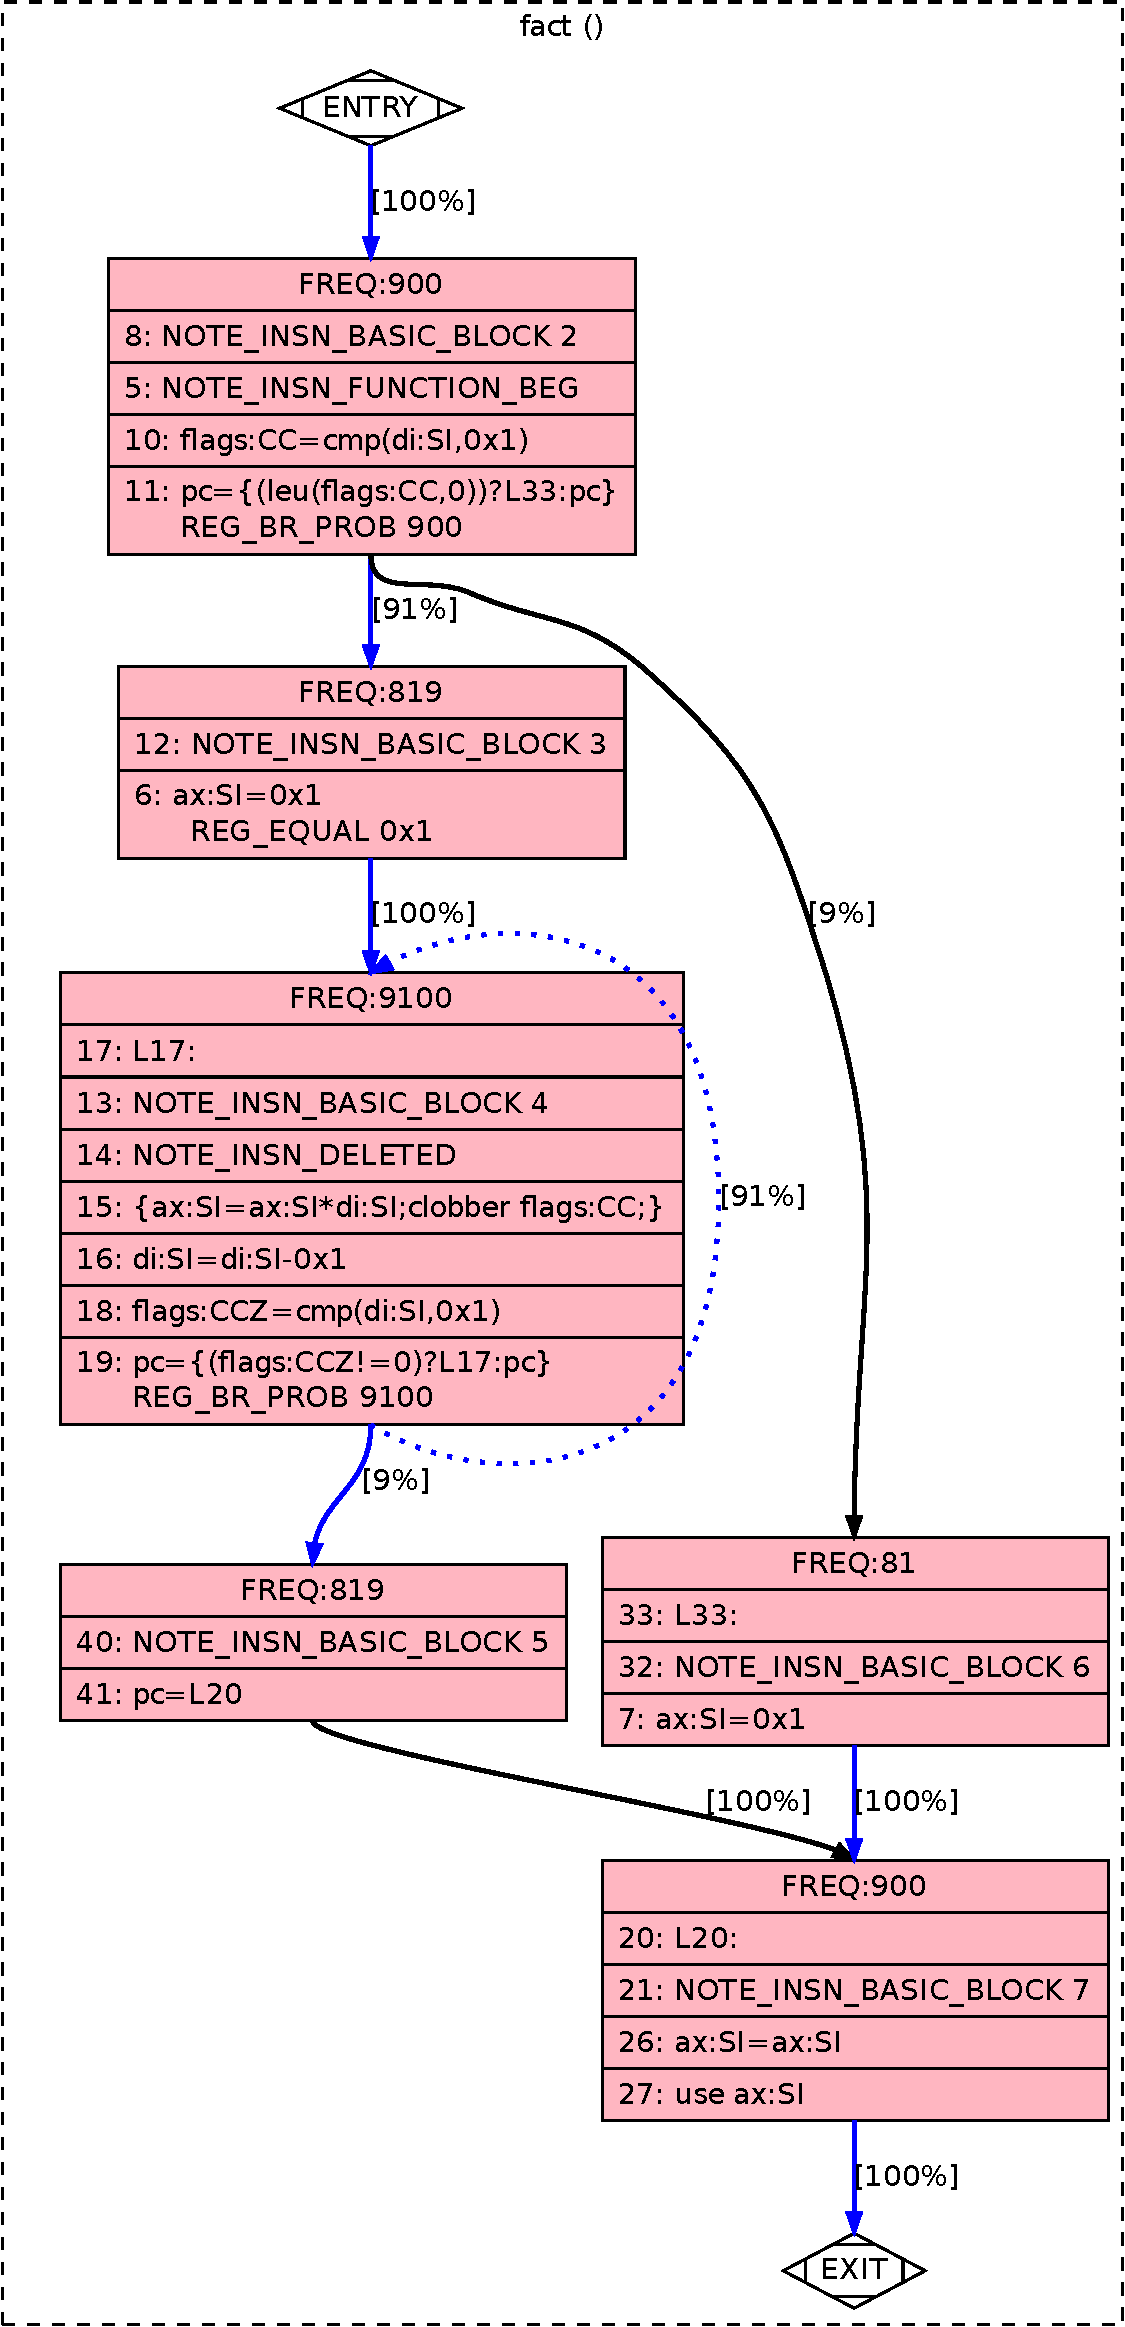
\includegraphics[height=0.7\textheight]{illustrations/fact-reloaded-crop.pdf}
\caption{RTL с физическими регистрами}
\label{fig:fact_rtl_reload}
\end{figure}

\subsubsection{Распределение регистров и кодогенерация}\label{subsubsec:PRTrans}

После выполнения преобразований на виртуальных регистрах, должен отработать распределитель регистров, который отображает виртуальные регистры в физические регистры, заданные в описании целевой архитектуры. Для x86 это ax, bx, cx, dx и так далее. Пример RTL с физическими регистрами приведен на рис \ref{fig:fact_rtl_reload}

Виртуальных регистров обычно больше чем физических, поэтому распределение регистров не может быть проведено один к одному, а должно использовать временные слоты в памяти для материализации (spilling) и последующего восстановления (filling) регистров.

Может показаться удивительным, но многие преобразования требуют представляения на физических регистрах, например расписание (scheduling) инструкций требует информации о конкретных задержках и модели конвейера и таким образом должно проводится только когда уже известно окончательное распределение переменных по регистрам и памяти в оптимизированном коде. Точно так же переименование регистров с целью облегчить регистровое давление бесполезно проводить на этапе виртуальных регистров, потому что там сам этот термин не имеет смысла.

После отработки оптимизаций на физических регистрах (if-conversion, переупорядочение базовых блоков, расписание инструкций), кодогенератор в GCC порождает ассемблер целевой архитектуры (в заданном синтаксисе).

В других компиляторах детали происходящего могут отличаться: в LLVM машинно-независимый IR очень похож на машинно-зависимый, в ICC промежуточное представление скрыто от пользователя и так далее. Но общая схема везде одна и та же: выскоуровневый IR (обычно машинно-независимый) преобразуется в машинно-зависимый IR среднего уровня, который после распределения регистров преобразуется в низкоуровневый IR. Который, в свою очередь, уже и используется для генерации кода.

\pagebreak
\subsection{Ассемблер}\label{subsec:Assembler}

Важно различать язык ассемблера как язык и ассемблер как программу. 

\begin{itemize}
\item \textbf{Язык ассемблера} это удобная символьная форма записи (мнемокод) команд и их аргументов
\item \textbf{Ассемблер} это программа, переводящая язык ассемблера в объектный код
\end{itemize}

Язык ассемблера целевой архитектуры задается документом, который называется Instruction Set Architecture (ISA) и является своим для каждой архитектуры. Более того, даже в пределах одной архитектуры могут существовать несколько синтаксисов языка ассемблера (пример -- AT\&T и Intel синтаксисы ассемблера x86).

\subsubsection{Ассемблирование}\label{subsubsec:Assembling}

Ассемблер как программа обрабатывает текстовый файл на языке ассемблера конкретной архитектуры и порождает объектный код для последующей линковки и исполнения.

В качестве примера, ассемблер (x86, синтаксис AT\&T), порождённый из функции факториал может выглядеть следующим образом:

\begin{verbatim}
  .file "fact.c"
  .section  .text.unlikely,"ax",@progbits
.LCOLDB0:
  .text
.LHOTB0:
  .p2align 4,,15
  .globl  fact
  .type fact, @function
fact:
.LFB0:
  .cfi_startproc
  cmpl  $1, %edi
  movl  $1, %eax
  jbe .L4
  .p2align 4,,10
  .p2align 3
.L3:
  imull %edi, %eax
  subl  $1, %edi
  cmpl  $1, %edi
  jne .L3
  rep; ret
.L4:
  rep; ret
  .cfi_endproc
.LFE0:
  .size fact, .-fact
\end{verbatim}

В нём можно выделить: 

\begin{itemize}
\item Инструкции x86: \lstinline!cmpl!, \lstinline!movl!, \lstinline!jbe!, \lstinline!imull!, \lstinline!subl! и прочие
\item Метки: \lstinline!fact!, \lstinline!LFB0!, \lstinline!L3!, \lstinline!L4!, \lstinline!LFE0!
Можно заметить, что одна из этих меток -- \lstinline!fact! объявлена глобальной, то есть попадёт в таблицу экспортируемых из этого модуля функций
\item Директивы: \lstinline!globl!, \lstinline!type!, \lstinline!size!, \lstinline!p2align!
\item Отладочную информацию: \lstinline!cfi_startproc!, \lstinline!cfi_endproc!
\item Секции \lstinline!text!, \lstinline!text.unlikely!
\end{itemize}

Ассемблер выполняет следующую работу:

\begin{enumerate}
\item Кодирование инструкций
\item Подстановка абсолютных значений переходов (где они известны) вместо символьных меток
\item Ассемблирование секций (кода, данных, стека)
\item Исполнение директив ассемблера (выравнивание, отладочная информация, прочее)
\item Формирование таблиц экспорта
\end{enumerate}

\subsubsection{Макроассемблер}

Почти любой ассемблер (включая ml.exe от Microsoft, GNU AS, а также отдельные распространённые ассемблеры, такие как wasm и nasm) поддерживает не только свои основные функции по обработке выдачи компилятора, но также предоставляет определенные средства для разработки собственно на языке ассемблера. В современном мире чистая разработка на ассемблере это экзотика, но она может быть нужна для работы с системными регистрами, использовании специфичных возможностей архитектуры и так далее -- в общем для всего, чего нельзя написать на C.

Препроцессор ассемблера обычно позволяет:

\begin{itemize}
\item Объявлять и использовать макросы. Например приведенный ниже макрос для GNU AS:

\begin{verbatim}
.macro  sum from=0, to=5
  .long   \from
  .if     \to-\from
  sum     "(\from+1)",\to
  .endif
.endm
\end{verbatim}

При вызове \lstinline!SUM 0,5! раскроется в:
 
\begin{verbatim}
  .long   0
  .long   1
  .long   2
  .long   3
  .long   4
  .long   5
\end{verbatim}

\item Включать ассемблерный код из других файлов (директива \lstinline!.include "file"! в GNU as или аналогичные ей).
\item Писать комментарии. Стили комментирования очень разнообразны и отличаются от ассемблера к ассемблеру. Большинство ассемблеров также поддерживают комментарии в стиле C.
\item Также поддерживаются дополнительные (иногда -- удивительно разнообразные) возможности. Так например в GNU as символ точка обозначает адрес текущей ассемблируемой инструкции. Поэтому запись:

\begin{verbatim}
melvin: .long .
\end{verbatim}

Обозначает, что метка melvin содержит собственный адрес.
\end{itemize}

Кроме общих для всех архитектур возможностей ассемблера в рамках его синтаксиса, каждая архитектура может определять набор своих средств для задания адресов в памяти, обращения к регистрам и так далее.

\subsubsection{Дизассемблирование}\label{subsubsec:Disasm}

Результатом работы ассемблера является объектный файл, который, в свою очередь, может быть дизассемблирован, то есть переведен обратно в ассемблерное представление. В случае GNU toolchain соответствующая утилита называется objdump. 

\begin{verbatim}
$ as fact.s -o fact.o
$ objdump -d fact.o
\end{verbatim}

Ниже рассмотрен вывод ассемблированного и сразу же дизассемблированного кода:

\begin{verbatim}
   0:	83 ff 01             	cmp    $0x1,%edi
   3:	b8 01 00 00 00       	mov    $0x1,%eax
   8:	76 13                	jbe    1d <fact+0x1d>
   a:	66 0f 1f 44 00 00    	nopw   0x0(%rax,%rax,1)
  10:	0f af c7             	imul   %edi,%eax
  13:	83 ef 01             	sub    $0x1,%edi
  16:	83 ff 01             	cmp    $0x1,%edi
  19:	75 f5                	jne    10 <fact+0x10>
  1b:	f3 c3                	repz retq 
  1d:	f3 c3                	repz retq 
\end{verbatim}

Дизассемблер аннотирован кодировкой (ниже будут рассмотрены способы аннотировать дизассемблер многим другим, в том числе номерами строк и даже самими строчками исходного кода программы).

Кроме того видно, что две p2align директивы породили выравнивающий nop.

\pagebreak
\subsection{Линкер}\label{subsec:Linker}

Линкер это программа, предназначенная для связывания (linking) нескольких объектных файлов в один исполняемый. Линкер входит во все известные наборы средств разработки -- в случае GCC он называется ld (или gold, это улучшенная версия ld от Google), в случае Microsoft это link.exe, есть и другие варианты линкеров. В случае LLVM, конкретная архитектура может реализовать свой линкер как библиотеку или использовать из-под драйвера вызов любого существующего линкера.

\subsubsection{Объявления и определения}\label{subsubsec:DeclDef}

Прежде чем переходить к рассмотрению линкера, необходимо расширить тестовую задачу. Пусть функция \lstinline!fact! физически находится в файле \lstinline!fact.c! и кроме него есть файл \lstinline!main.c!, задача которого -- распечатать факториал пяти, выполнив для этого строчку вроде следующей:

\begin{lstlisting}
printf ("%d\n", fact(5));
\end{lstlisting}

Но откуда вообще компилятор при обработке файла \lstinline!main.c! узнает что такое \lstinline!fact! и что такое \lstinline!printf!? Для того, чтобы какая-то функция могла быть использована на этапе компиляции, она должна быть \textbf{объявлена} -- то есть указано её имя, типы её аргументов и тип возвращаемого значения. Обычно объявления собираются вместе в заголовочные файлы. Есть стандартные заголовочные файлы, такие, как \lstinline!stdio.h!, содержащий объявление функции \lstinline!printf!. Для факториала, заголовочный файл \lstinline!fact.h! может выглядеть как-то так:

\begin{lstlisting}
#ifndef FACT_GUARD_
#define FACT_GUARD_

extern unsigned fact (unsigned);

#endif
\end{lstlisting}

Теперь программа, распечатывающая факториал может быть написана как-то так:

\begin{lstlisting}
#include <stdio.h>
#include "fact.h"

int
main (void)
{
  printf ("%d\n", fact(5));
  return 0;
}
\end{lstlisting}

Этот файл использует функцию, которая \textbf{определена} в другом месте -- в данном случае в файле \lstinline!fact.c!. Если попытаться сделать исполняемый файл из одного \lstinline!main.c!, это завершится ошибкой:

\begin{verbatim}
$ gcc main.c
/tmp/ccunVXEF.o: In function `main':
main.c:(.text+0xa): undefined reference to `fact'
collect2: ld returned 1 exit status
\end{verbatim}

Компилятор видит тип функции \lstinline!fact! и знает как её вызвать, но линкер не может разрешить этот вызов. Можно сказать, что в коде на C, объявления пишутся для компилятора (достаточны чтобы сгенерировать в ассемблере вызов на внешнюю метку), а определения для линкера (достаточны для разрешения этой метки в программе, состоящей из множества единиц трансляции). 

Простейший способ успешно скомпилировать искомую программу успешно это подать оба файла драйверу:

\begin{verbatim}
$ gcc main.c fact.c
\end{verbatim}

Но что и в каком порядке при этом будет сделано?

\begin{itemize}
\item Будут скомпилированы отдельно \lstinline!main.c! и \lstinline!fact.c! до ассемблера (временные файлы будут скорее всего сохранены куда-то в недоступное для глаз пользователя место).
\item Оба получившихся ассемблерных файла будут сассемблированы до объектного кода (скорее всего будет размещен там же)
\item Получившийся объектный код через специальный скрипт \lstinline!collect2! будет подан линкеру (в случае GNU Toolchain это \lstinline!ld! или \lstinline!gold!).
\end{itemize}

Как обычно опция \lstinline!-save-temps! позволяет сохранить промежуточные результаты работы.

\subsubsection{Статическая линковка}\label{subsubsec:Linking}

Существует два вида линковки -- статическая и динамическая. Де-факто стандартным умолчанием в большинстве средств разработки является динамическая линковка (и её преимущества, благодаря которым это так, тоже будут рассмотрены). Но статическая линковка гораздо проще для объяснения, поэтому следует начать с неё. Статически слинкованный пример с сохранёнными временными файлами можно получить следующим образом.

\begin{verbatim}
$ gcc main.c fact.c -static --save-temps
\end{verbatim}

Или с явным вызовом \lstinline!ld! и сохранением порядка секций:

\begin{verbatim}
$ gcc main.c -c
$ gcc fact.c -c
$ ld -static main.o fact.o
\end{verbatim}

Для исследования происходящего (под Linux) удобна утилита \lstinline!readelf! из набора бинарных утилит. Анализироваться ниже будет её вывод с опцией \lstinline!readelf -s!. Можно увидеть, что для объектного файла \lstinline!main.o! список функций выглядит как-то так:

\begin{verbatim}
     9: 0000000000000000    43 FUNC    GLOBAL DEFAULT    1 main
    10: 0000000000000000     0 NOTYPE  GLOBAL DEFAULT  UND fact
    11: 0000000000000000     0 NOTYPE  GLOBAL DEFAULT  UND printf
\end{verbatim}

Здесь одна глобальная метка \lstinline!main! и две не разрешенных \lstinline!fact! и \lstinline!printf!. Теперь для объектного файла \lstinline!fact.o!:

\begin{verbatim}
     8: 0000000000000000    43 FUNC    GLOBAL DEFAULT    1 fact
\end{verbatim}

можно увидеть, что определение этой функции в нём есть. При статической линковке, линкер собирает все объектные файлы и разрешает их метки относительно друг друга в адресах получившегося общего файла. В итоге для результата \lstinline!a.out! картина выглядит так:

\begin{verbatim}
   901: 0000000000401740   157 FUNC    GLOBAL DEFAULT    6 printf
  1545: 0000000000400434    43 FUNC    GLOBAL DEFAULT    6 main
  1833: 0000000000400460    43 FUNC    GLOBAL DEFAULT    6 fact
\end{verbatim}

Здесь во второй колонке указаны адреса в объектном файле и те же адреса можно увидеть в дизассемблере (всё так же \lstinline!objdump -d! для GNU Toolchain ну или ваш любимый дизассемблер в вашей системе).

\begin{verbatim}
0000000000400434 <main>:
  400434: 55                    push   %rbp
  400435: 48 89 e5              mov    %rsp,%rbp
  400438: bf 05 00 00 00        mov    $0x5,%edi
  40043d: e8 1e 00 00 00        callq  400460 <fact>
  400442: 89 c2                 mov    %eax,%edx
....
0000000000400460 <fact>:
  400460: 55                    push   %rbp
  400461: 48 89 e5              mov    %rsp,%rbp
....
\end{verbatim}

Можно заметить, что в кодировку инструкции \lstinline!сall! (в x86 ассемблере это \lstinline!e8!) подставлено относительное смещение \lstinline!1e!, и действительно (дисплейсмент вызова считается относительно начала следующей инструкции) получается, что \lstinline!400442 + 1e = 400460!.

В этом суть статической линковки: объектный код объединяется, разрешаются ссылки и ссылки подставляются всюду, в том числе и в ассемблерные инструкции такие как \lstinline!call!. Если посмотреть дизассемблер объектного (ещё не не слинкованного) файла, можно увидеть, что вызов там не разрешён. В конкретный адрес, вместо этого подставлены нули:

\begin{verbatim}
0000000000000000 <main>:
   0: 55                    push   %rbp
   1: 48 89 e5              mov    %rsp,%rbp
   4: bf 05 00 00 00        mov    $0x5,%edi
   9: e8 00 00 00 00        callq  e <main+0xe>
   e: 89 c2                 mov    %eax,%edx
\end{verbatim}

Это интерпретируется как вызов с передачей управления на следующую инструкцию. Но это конечно не так, речь просто о не подставленной на этом этапе \textbf{релокации}. Релокацией (relocation information или попросту релоком) называется метаинформация в объектном файле обо всех местах, куда линкер должен подставить адреса при линковке.

Информацию о релокациях можно считать из объектного файла:

\begin{verbatim}
readelf -r main.o
00000000000a  000a00000002 R_X86_64_PC32  00000000 fact - 4
000000000011  00050000000a R_X86_64_32    00000000 .rodata + 0
000000000020  000b00000002 R_X86_64_PC32  00000000 printf - 4
\end{verbatim}

Первая в этом списке (по адресу \lstinline!0xa!) это и есть та самая, которая должна быть подставлена в \lstinline!call!, а конкретно \lstinline!fact! минус размер инструкции вызова.

Хорошо, допустим с \lstinline!fact! всё понятно. Но где посмотреть объектник, который используется при линковке с функцией \lstinline!printf!? Здесь не всё так очевидно, потому что эта функция берётся из \textbf{библиотеки}.

\subsubsection{Статические библиотеки}\label{subsubsec:StaticLibs}

Статическая библиотека (static library) это способ организации объектного кода, при котором большое число раздельно сассемблированных файлов заменяется одним, объединяющим их все и также содержащим некую метаинформацию.

В MSVS собрать статическую библиотеку можно настроив опции линковщика, в то время, как в GNU Toolchain, для этого есть отдельная утилита, называющаяся \lstinline!ar!. На примере уже рассмотренного факториала, можно собрать статическую библиотеку из одного модуля:

\begin{verbatim}
ar -cr libfact.a fact.o
\end{verbatim}

В конце этой строки можно указать сколько угодно объектных файлов и все они будут объединены (также говорят -- упакованы) в одну библиотеку. Ей можно пользоваться непосредственно:

\begin{verbatim}
gcc -static main.c libfact.a
\end{verbatim}

Но общепринятый способ использования -- указание пути и сокращенного имени, которые достаточны драйверу, чтобы сформировать для линкера полное имя:

\begin{verbatim}
gcc -static -L. main.c -lfact
\end{verbatim}

Также конвенциальным является сокращение \lstinline!libxxx.a! в записи аргументов командной строки до \lstinline!-lxxx!. Например \lstinline!libm.a! записывается как \lstinline!-lm!, а \lstinline!libс.a! как \lstinline!-lс!. Именно таким образом на сборку подаются все стандартные библиотеки, причем даже если их явно не указать. Так например запустив указанную выше строчку с дополнительной опцией \lstinline!verbose!, можно увидеть окончательную строчку вызова линкера вида:

\begin{verbatim}
collect2 -m elf_x86_64 -static crtbeginT.o -L. 
-L<other paths here> main.o -lfact --start-group 
-lgcc -lgcc_eh -lc --end-group crtend.o crtn.o
\end{verbatim}

Видно, что драйвер тихо добавил в опции линкера несколько стандартных библиотек и объектных файлов, в частности libc, откуда и берется определение для функции \lstinline!printf!.

Ту же утилиту, которая отвечает за создание библиотек, можно использовать и для исследования библиотек. Например вот так можно распечатать все объектные файлы из которых собрана \lstinline!libc!:

\begin{verbatim}
ar -vt /usr/lib/libc.a
\end{verbatim}

\subsubsection{Динамическая линковка}\label{subsec:DynLink}

Статические библиотеки хороши и просты, но у них есть недостатки:

\begin{itemize}
\item Большой размер файла на диске
\item Тратится много памяти при исполнении нескольких файлов, использующих одну и ту же библиотеку
\end{itemize}

Чтобы преодолеть эти проблемы, используется динамическая линковка. В этом случае, код из библиотеки связывается с кодом использующей её программы только после того, как программа загружена. 

Всё, что будет сказано ниже актуально для Unix-подобных систем. В случае Windows, динамические библиотеки (так называемые DLL) работают несколько иначе, например там нет настоящего позиционно-независимого кода и всего такого.

Сборка в динамическую библиотеку с помощью GNU Toolchain под OS Linux проходит в два этапа:

\begin{verbatim}
gcc -c -fPIC -O2 fact.c
gcc -shared fact.o -o libfact.so
\end{verbatim}

Опция \lstinline!-fPIC! определяет необходимость сассемблировать код так, чтобы он был positional-independent, то есть не содержал прямых вызовов функций. На примере \lstinline!main.c! можно посмотреть типичный positional-independent ассемблер:

\begin{verbatim}
main:
  subq  $8, %rsp
  movl  $5, %edi
  call  fact@PLT
...
\end{verbatim}

Отметка \lstinline!@PLT! здесь сообщает о необходимости сгенерировать вызов fact относительно PLT (procedure linkage table). На (рис. \ref{fig:dl}) показана общая схема работы.

\begin{figure}[ht]
\centering
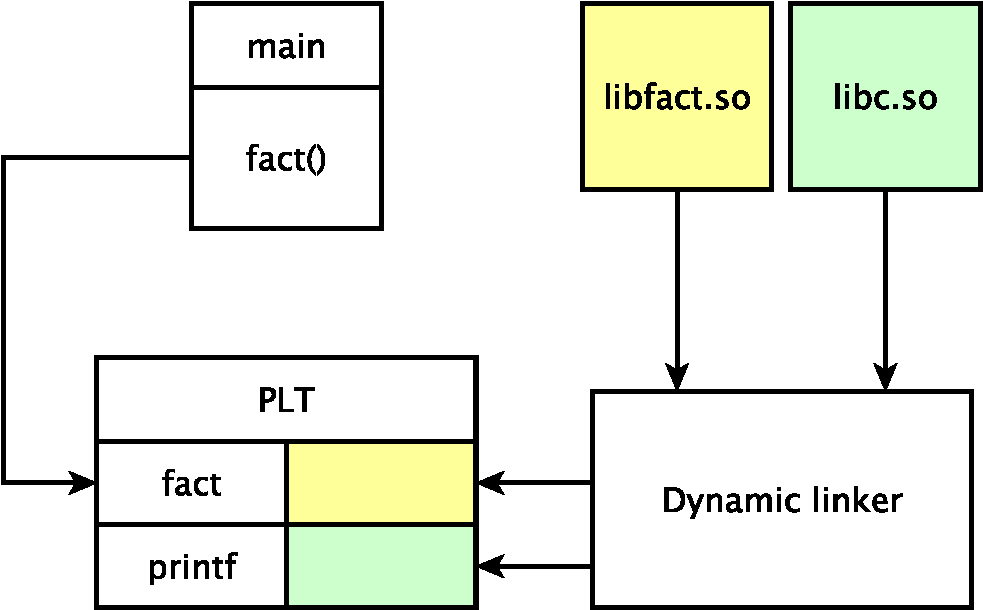
\includegraphics[width=0.8\textwidth]{illustrations/dl-scheme-crop.pdf}
\caption{Динамическая линковка}
\label{fig:dl}
\end{figure}

Окончательное связывание вызываемой функции с её точой входа в таблице PLT осуществляется сравнительно поздно специальной программой, известной как динамический линкер (dynamic linker). Часто на него ссылаются по его типичному имени \lstinline!ld.so!.

Для данных, прямые ссылки на которых тоже неизвестны на этапе линковки, существует GOT -- global offset table, которая тоже заполняется динамическим линкером уже после загрузки программы.

\subsubsection{Динамические и смешанные библиотеки}\label{subsubsec:Mixlib}

После того, как \lstinline!libfact.so! построена, использовать её для сборки кода с ней не сложнее, чем в случае статических библиотек.

\begin{verbatim}
gcc -fPIC main.c -L. -lfact -Wl,-rpath,.
\end{verbatim}

Драйвер достаточно умён, чтобы в случае динамической сборки заменить короткое имя \lstinline!-lxxx! на \lstinline!libxxx.so!, как в случае с \lstinline!-lfact! выше.

Поскольку динамические библиотеки не объединяются с кодом исполняемого файла, они должны лежать отдельно (и лежать по правильным путям). Выше опция \lstinline!-rpath! указывает начинать поиск зависимостей с текущей папки. Она подаётся под специальным флажком \lstinline!Wl!, который прокидывает все свои опции непосредственно линкеру, минуя обычную обработку драйвером. Аналогичный флажок \lstinline!Wa! существует и для ассемблера.

В слинкованную программу, строчки поиска динамических библиотек записываются как метаинфрмация (зависимости). Чтобы посмотреть все зависимости того или иного файла можно использовать специальную утилиту ldd:

\begin{verbatim}
$ ldd a.out 
	linux-vdso.so.1 =>  (0x00007fff6956b000)
	libfact.so => ./libfact.so (0x00007f86adf83000)
	libc.so.6 => /lib/libc.so.6 (0x00007f86adbd2000)
	/lib64/ld-linux-x86-64.so.2 (0x00007f86ae186000)
\end{verbatim}

Видны зависимости от динамического линкера, libc, и libfact, а также зависимость от vdso -- это системный механизм Linux.

Динамические библиотеки имеют свои недостатки:

\begin{itemize}
\item Каждый вызов идёт по косвенности, что заставляет платить за него дополнительный переход
\item Программа может не заработать если библиотеки будут не найдены или лежать по неправильным путям
\end{itemize}

В случае крупных блиблиотек, таких как libc, достоинства с лихвой перекрывают недостатки. Но в случае факториала, хорошо бы прилинковать его статически, оставив libc по возможности динамической. Такая возможность есть почти во всех тулчейнах, в GNU Toolchain она реализуется логическими скобками Bstatic/Bdynamic.

\begin{verbatim}
gcc test.c -Wl,-Bstatic -lfact -Wl,-Bdynamic -L.
\end{verbatim}

Здесь факториал будет прилинкован статически, а всё остальное, что линкер подставит по умолчанию будет линковаться динамически.

\pagebreak
\subsection{Уточнения}\label{subsec:Amendments}

Прежде чем двигаться дальше, полезно ещё раз окинуть взглядом ту общую картину которая пока что получилась.

На (рис. \ref{fig:toolchain_completed}) представлена схема системы компиляции, более подробная, по сравнению с (рис. \ref{fig:simplified_scheme}) и гораздо более реалистичная.

\begin{figure}[ht]
\centering
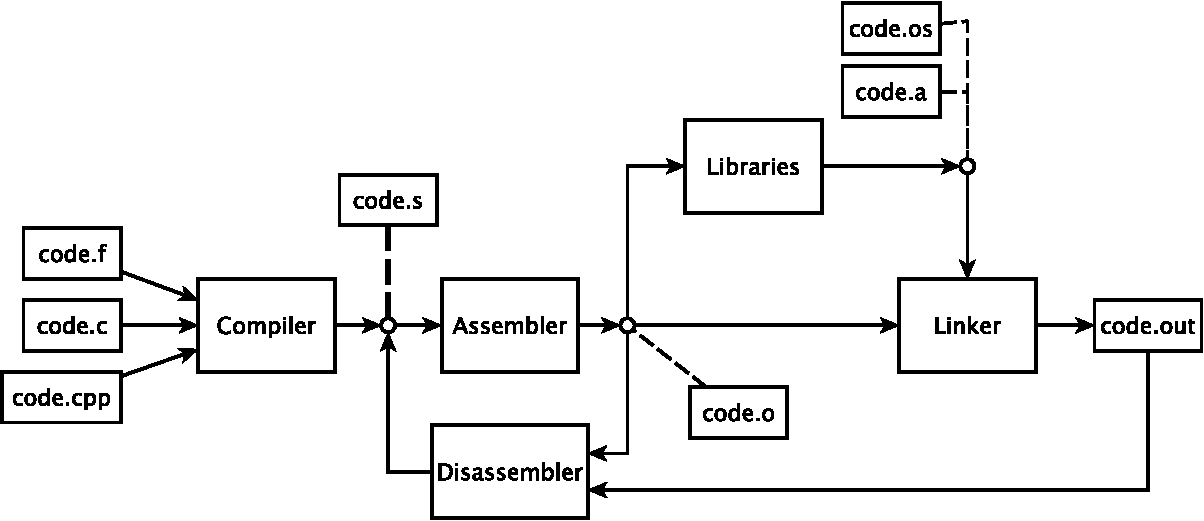
\includegraphics[width=1.0\textwidth]{illustrations/mipt-scheme-crop.pdf}
\caption{Уточненная схема toolchain}
\label{fig:toolchain_completed}
\end{figure}

На этой схеме всё ещё не отображены:

\begin{itemize}
\item Большинство бинарных утилит
\item Стандартные библиотеки
\item Средства отладки и профилировки
\end{itemize}

Далее все эти дополнительные средства будут разобраны подробно.

\subsubsection{Форматы исполняемых файлов}\label{subsubsec:ELF}

Финальным результатом работы системы компиляции являются, как видно из (\ref{fig:toolchain_completed}) исполняемые или объектные файлы. На самом деле форматов этих файлов тоже бывает достаточно много и хороший линкер может порождать файлы разных форматов в зависимости от требований пользователя.

Наиболее известные форматы файлов:

\begin{itemize}
\item a.out -- древний, но всё ещё популярный за свою минималистичность формат (в качестве исполняе)
\item ELF -- де-факто стандарт для исполняемого и объектного кода в Unix-подобных системах
\item PE -- де-факто стандарт (включая свою доработку PE32+) в исполняемого кода Windows-подобных системах
\item COFF -- популярен (как и его доработка ECOFF) для объектных файлов
\end{itemize}

Далее будет предполагаться что везде речь идёт именно об ELF файлах.

\begin{figure}[ht]
\centering
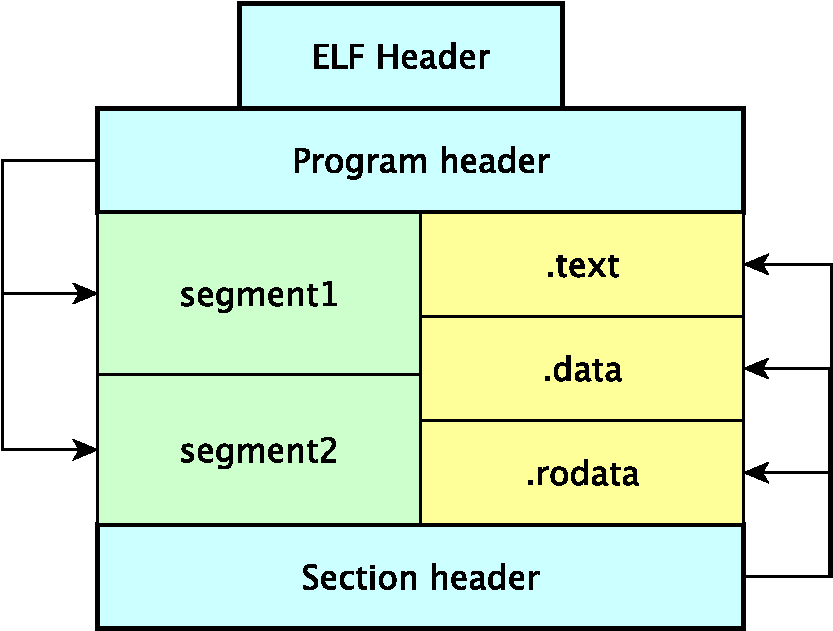
\includegraphics[width=0.6\textwidth]{illustrations/elf-structure-crop.pdf}
\caption{Формат ELF файла}
\label{fig:elf}
\end{figure}

ELF это аббревиатура от "Executable and Linkable Format", изначально он был разработан и опубликован компанией USL как часть двоичного интерфейса приложений операционной системы UNIX System V. Каждый такой файл имеет два заголовка: program header, описывающий сегменты файла и section header, описывающий секции файла.

Сегменты являются информацией для загрузчика, в то время как секции являются информацией для линкера. Сегменты и секции могут пересекаться (и обычно пересекаются, как это изображено на рис. \ref{fig:elf}), но в файле могут быть также и байты не относящиеся ни к одной секции.

\pagebreak
\section{Вокруг toolchain}\label{sec:AroundToolchain}

Системы компиляции не существуют в одиночестве. Программу мало скомпилировать, сассемблировать и слинковать, жизненный цикл современного ПО требует отладки, профилировки, поддержки со стороны стандартных библиотек.

\subsection{Стандартная библиотека}\label{subsec:Library}

Стандарты большинства современных языков программирования регламентируют поставку вместе с компилятором языка так называемой ``стандартной библиотеки'' -- набора часто используемых подпрограмм с хорошо документированным поведением.

Классикой жанра является стандартная библиотека языка C. Можно перечислить несколько разновидностей:

\begin{itemize}
\item GNU C Library – самая распространенная реализация, используемая в Linux
\item Microsoft C Run-time Library
\item Dietlibc – альтернативная небольшая реализация Стандартной библиотеки Си
\item uClibc – Стандартная библиотека Си для встраиваемых систем на базе Linux
\item Newlib – Стандартная библиотека языка Си для встраиваемых систем
\item Klibc – применяется главным образом для загрузки Linux-систем
\item Eglibc – разновидность glibc для встраиваемых систем
\item bionic – реализация стандартной библиотеки в Android
\end{itemize}

Обычные требования к стандартной библиотеке: стабильность и качество реализации библиотечных подпрограмм, максимальное использование специфики архитектуры.

Хороший пример: функция \lstinline!strcpy!. Её настоящая реализация в той же glibc для x86 очень существенно отличается от наивного подхода изложенного в K\&R. Обычно каждая функция в стандартной библиотеке для каждой архитектуры это результат многолетнего и кропотливого труда программистов и аналитиков.

\pagebreak
\subsection{Бинарные утилиты}\label{subsec:Binutils}

Многие бинарные утилиты уже были рассмотрены выше, но здесь можно привести полный список бинарных утилит GNU Toolchain (он почти не отличается от такого же списка для LLVM toolchain и имеет некоторые, но не концептуальные отличия от тех утилит, которые доступны под Windows).

Некоторые бинарные утилиты уже рассматривались выше:

\begin{itemize}
\item as -- ассемблер, рассматривался в (\ref{subsubsec:Assembling})
\item objdump -- дизассемблер, рассматривался в (\ref{subsubsec:Disasm})
\item ld -- линкер, рассматривался в (\ref{subsubsec:Linking})
\item readelf -- упоминался в (\ref{subsubsec:Linking})
\item ar -- упаковщик статических библиотек, упоминался в (\ref{subsubsec:Linking})
\end{itemize}

Другие пока не так хорошо знакомы и будут рассмотрены далее 

\subsubsection{addr2line}\label{subsubsec:AddrLine}

Очень часто при запуске плохо отлаженной программы, можно получить segfault, неприятного вида. Синтетический пример:

\begin{lstlisting}
int main()
{
  int *p = (int*)0xDEADBEEF;
  *p = 5; /* boom */
}
\end{lstlisting}

При запуске даёт:

\begin{verbatim}
$ gcc segf.c
$ ./a.out 
Segmentation fault
$ dmesg | tail -1
[ 4051.415509] a.out[3346]: segfault at deadbeef 
ip 00000000004004da sp 00007fffdd0a97c0 error 6 in a.out[400000+1000]
\end{verbatim}

Если программа большая, может быть не вполне ясно чему соответствует адрес $4004da$. В этом случае можно собрать ту же программу с отладочной информацией и узнать номер строки по адресу:

\begin{verbatim}
$ gcc -g segf.c
$ addr2line -e a.out 0x00000000004004da
segf.c:4
\end{verbatim}

Что сразу даёт информацию о том, что ошибка в четвертой строке и может сделать отладку гораздо проще.

\subsubsection{c++filt}\label{subsubsec:Demangle}

Деманглер иногда оказывается крайне полезен. Для того, чтобы сделать возможными функции-члены в структурах, перегрузку функций и пространства имён, C++ искажает имена функций, в результате чего в ассемблере целевой архитекутры они мало читаемы:

\begin{verbatim}
_ZSt4endlIcSt11char_traitsIcEERSt13basic_ostreamIT_T0_ES6_
\end{verbatim}

Всегда страшно встретить нечто такое. Но простое использование здесь деманглера позволяет получить (расшифровать?) точное имя этой метки в C++ коде:

\begin{lstlisting}
std::basic_ostream<char, std::char_traits<char>>& 
std::endl<char, std::char_traits<char>> (
  std::basic_ostream<char, std::char_traits<char>>&)
\end{lstlisting}

Откуда видно, что это просто \lstinline!std::endl! -- стандартный способ указать конце строки при выводе в C++.

К сожалению, правила манглирования имён не регламентируются никакими стандратными документами, поэтому деманглер одной архитектуры скорее всего не подойдет для любой другой.

\subsubsection{elfedit и objcopy}\label{subsubsec:Objcopy}

Утилита elfedit используется для редактирования метаданных в ELF-файлах. Во многих отношениях она дополняет readelf, который позволяет только анализировать файлы, возможностями редактирования.

Формат ELF играет громадную роль в GNU Toolchain и в Linux, но его использование за их пределами ограничено, поэтому нет смысла здесь углубляться в детали.

Гораздо более распространена утилита objcopy, которая позволяет делать удивительные вещи: например создавать объектный файл, готовый для линковки с кодом на C практически из любого бинарного мусора

\begin{verbatim}
$ dd if=/dev/urandom of=blob.bin bs=1 count=16
$ objcopy -I binary -O elf64-x86-64 -B i386 blob.bin blob.o
$ objdump -t blob.o
blob.o:     file format elf64-x86-64
SYMBOL TABLE:
00000000 l    d  .data	00000000 .data
00000000 g       .data	00000000 _binary_blob_bin_start
00000010 g       .data	00000000 _binary_blob_bin_end
00000010 g       *ABS*	00000000 _binary_blob_bin_size
\end{verbatim}

Теперь в C коде можно использовать эти метки как нормальные объявления

\begin{lstlisting}
extern unsigned char _binary_blob_bin_start;
extern unsigned char _binary_blob_bin_end;
extern unsigned char _binary_blob_bin_size;
/* .... */
unsigned char *pblob = &_binary_blob_bin_start;
\end{lstlisting}

Разумеется мусор тут взят только для примера. Линковка в программу любых ресурсов, в том числе самых причудливых, средствами objcopy не сложнее.

\subsubsection{nm и objdump}

Утилита nm является упрощением objdump для posix-подсистем и всё, что умеет nm можно сделать через objdump. До сих пор objdump рассматривался только как дизассемблер, но эта пара умеет гораздо больше. Так например стандартная фича nm (она же используется через objdump -t) это просмотр таблицы имён.

\begin{verbatim}
$ nm test.o
                 U fact
0000000000000000 T main
                 U printf
\end{verbatim}

Здесь видны два неопределенных имени (fact и printf). Objdump покажет больше информации:

\begin{verbatim}
$ objdump -t test.o

test.o:     file format elf64-x86-64

SYMBOL TABLE:
0000000000000000 l    d  .text	0000000000000000 .text
0000000000000000 l    d  .data	0000000000000000 .data
0000000000000000 l    d  .bss	0000000000000000 .bss
0000000000000000 l    d  .rodata	0000000000000000 .rodata
....
0000000000000000 l    d  .comment	0000000000000000 .comment
0000000000000000 g     F .text	0000000000000026 main
0000000000000000         *UND*	0000000000000000 fact
0000000000000000         *UND*	0000000000000000 printf
\end{verbatim}

Видны также все секции, каждую из которых можно посмотреть отдельно.

\subsubsection{strip}\label{subsubsec:Strip} 

Полезная утилита strip используется для вырезания символьной и отладочной информации и оптимизации размера файла:

\begin{verbatim}
$ du -b fact.o
1232	fact.o
$ strip fact.o -o fact-s.o
$ du -b fact-s.o
832	fact-s.o
\end{verbatim}

Как видно для простого объектного файла, содержащего только функцию факториал, его размер был уменьшен в полтора раза. Увы, цена этого уменьшения велика. Например теперь оттуда ничего нельзя прчоитать командой nm:

\begin{verbatim}
$ nm fact-s.o
nm: fact-s.o: no symbols
\end{verbatim}

Поэтому имеет смысл использовать strip с осторожностью только для уже отлаженного и гарантированно работающего кода.

\pagebreak
\subsection{Отладчики и отладка}\label{subsec:Debugger}

Важным этапом жизненного цикла программы является её отладка, когда возможен контроль её состояния в пошаговом режиме, включая как низкоуровневый контроль (считать регистры, память, исполнить один ассемблерный шаг), так и довольно высокоуровневый, включающий построчное выполнение кода и просмотр состояния переменных.

Большинство современных процессоров поддерживают возможности для отладки для аппаратном уровне, например возможность пошагового исполнения часто реализуется как trap flag, аппаратная поддержка точек останова и наблюдения через специальные прерывания, поддержка специальных отладочных протоколов самого процессора, таких так JTAG, etc.

\subsubsection{Обзор отладчиков}\label{subsubsec:Overview}

Отладчики делятся по уровню работы на:

\begin{itemize}
\item Отладчики микроархитектуры, такие как OpenOCD (on-chip debugger), способные работать непосредственно с процессором, с полным доступом к его системным регистрам и памяти, исполняются обычно вне отлаживаемого устройства, подключаясь к нему по протоколу, такому как JTAG

\item Отладчики уровня ядра, такие как KGDB или WinDbg, позволяют отлаживать операционную систему: имеют доступ к системным регистрам и физической памяти, исполняются как привилегированный код, но чаще уже на самом устройстве.

\item Отладчики пользовательского уровня, такие как GDB, LLDB, IDB, MSVS Debugger и многие другие: исполняются с правами обычного пользователя и имеют непривилегированный доступ к виртуальной памяти отлаживаемого процесса.
\end{itemize}

Отладчики первых двух типов бывают очень интересны, но обычно обладают урезанными возможностями и являются инструментами профессионалов со всеми присущими ограничениями. Далее речь пойдет в основном про GDB и более простую отладку уровня пользователя.

\subsubsection{Работа с GDB}\label{subsubsec:GDB}

Проще всего научится отлаживать программы отлаживая программы. 

Пусть дан на первый взгляд обычный вариант пузырьковой сортировки.

\begin{lstlisting}
/* Simple but buggy bubble sort  *
 * Can you find the bugs?        */
void 
sort(item *a, int n) 
{ 
  int i = 0, j = 0;
  int s;

  for (; i < n && s != 0; i++) 
    {
      s = 0;
      for (j = 0; j < n; j++) 
        if (a[j].key > a[j+1].key)   
          {
            item t = a[j];
            a[j] = a[j+1];
            a[j+1] = t;
            s++;
          }
      n--;
    }
}
\end{lstlisting}

Сколько проблем в таком коде можно найти пристально вглядываясь в него? Вряд ли много. Чтобы начать отладку, программу следует откомпилировать с отладочной информацией и запустить под отладчиком:

\begin{verbatim}
$ gcc buggy-sort.c -g -o buggy
\end{verbatim}

Здесь хорошо выучить несколько наиболее распространенных команд gdb:

\begin{verbatim}
help – list commands 
run – start your program [with arglist if needed] 
list – show lines of source 
break – set a break point in your code 
next – execute next line, stepping over function calls 
step – execute next line, stepping into function calls 
print – print the contents of variables and data structures 
frame – select frame number, point to the stack you are interested in 
backtrace – display program stack and control flow 
command – execute GDB command-list every time breakpoint n is reached 
cont – continue the execution of the code 
quit – quit the debugger
\end{verbatim}

Далее лучше делать с проектором вместе со студентами:

\begin{verbatim}
(gdb) break sort
Breakpoint 1 at 0x40056f: file buggy-sort.c, line 23.
(gdb) run
Breakpoint 1, sort (a=0x601040, n=5) at buggy-sort.c:23
23	  int i = 0, j = 0;
(gdb) next
26	  for (; i < n && s != 0; i++) 
(gdb) print s
$1 = 0
\end{verbatim}

Видно, что переменная s должна быть инициализирована во что-то ненулевое. Но после инициализации переменной s, программа сортирует явно не слишком хорошо.

Тут надо в аудитории продолжить разбор и найти все ошибки. Читающему это как текстовый файл это может быть оставлено как домашнее задание.

\subsubsection{Отладочная информация}\label{subsubsec:DWARF}

Отладочная информация, которая позволяет делать все вышеперечисленное. 

Существует много форматов отладочной информации:

\begin{itemize}
\item OMF -- ранее популярный, но устаревший формат для ранних DOS-подобных систем
\item DWARF -- де-факто стандарт отладочной информации в Unix-подобных системах
\item PE/COFF -- де-факто стандарт отладочной информации в Windows-подобных системах
\end{itemize}

Далее будет рассматриваться формат DWARF, названный так в пару к формату ELF исполняемых файлов.

Часть отладочной информации можно видеть в ассемблере:

\begin{verbatim}
fact:
.LFB0:
  .file 1 "fact.c"
  .loc 1 3 0
  .cfi_startproc
  pushq %rbp
.LCFI0:
  .cfi_def_cfa_offset 16
  movq  %rsp, %rbp
  .cfi_offset 6, -16
.LCFI1:
  .cfi_def_cfa_register 6
  subq  $16, %rsp
  movl  %edi, -4(%rbp)
  .loc 1 4 0
  cmpl  $1, -4(%rbp)
  ja  .L2
  .loc 1 5 0
  movl  $1, %eax
  jmp .L3
\end{verbatim}

Здесь специальные метки loc отмечают границы строк кода. 

\begin{lstlisting}
unsigned
fact (unsigned x)
{
  if (x < 2)
    return 1;

  return x * fact (x-8, 1);
}
\end{lstlisting}

Можно обратить внимание, что строка 3 это всего лишь открывающая фигурная скобка, но как много всего происходит между ней и строчкой 4!

Этот фрагмент кода называется \textbf{пролог} и можно ещё раз его повторить ниже:

\begin{verbatim}
  .loc 1 3 0
  .cfi_startproc
  pushq %rbp
.LCFI0:
  .cfi_def_cfa_offset 16
  movq  %rsp, %rbp
  .cfi_offset 6, -16
.LCFI1:
  .cfi_def_cfa_register 6
  subq  $16, %rsp
  movl  %edi, -4(%rbp)
  .loc 1 4 0
\end{verbatim}

В прологе происходит:

\begin{itemize}
\item Сохранение фрейм пойнтера (в данном случае регистр rbp) в стек.

\item Заполнение фрейм пойнтера стек пойнтером для того, чтобы отметить начало текущего фрейма в стеке.

\item Сдвиг вниз стек пойнтера чтобы дать место для локальных переменных
\end{itemize}

Отладочная информация зашифрованная в CFI (call frame information) метках, легко считывается визуально:

\begin{itemize}
\item \textbf{cfi\_startproc}

Обозначает начало текущей функции, точку входа, на которой остановится отладчик.

\item \textbf{cfi\_def\_cfa\_offset}

Устанавливает смещение CFA (canonical frame address) в это функции, отмечая место в котором на стеке сохранено значение указателя стека вызывающей процедуры.

\item \textbf{cfi\_offset}

Устанавливает, что предыдущее значение регистра 6 (то есть rsp) сохранено на указанном в offset (второй параметр) расстоянии от CFA.

\item \textbf{cfi\_def\_cfa\_register}

Модифицирует правило для вычисления CFA. Начиная от этой директивы для этого используется указанный как параметр регистр
\end{itemize}

Эта отладочная информация зависит от архитектуры по сути но не по формату. Тот же пролог для ARM, а не для x86 выглядит так:

\begin{verbatim}
  .loc 1 3 0
  .cfi_startproc
  stmfd sp!, {fp, lr}
  .cfi_def_cfa_offset 8
  .cfi_offset 11, -8
  .cfi_offset 14, -4
  add fp, sp, #4
  .cfi_def_cfa 11, 4
  sub sp, sp, #8
  str r0, [fp, #-8]
  .loc 1 4 0
\end{verbatim}

По сути он совсем другой, поскольку в мире ARM действуют иные соглашения о вызове и раскладке стека, но все CFI метки все так же отлично считываемы и ясны.

Кроме того, много отладочной информации зашифровано в  специальных секциях. Её можно исследовать с помощью \textbf{objdump} с опцией dwarf и указанием того, какую именно отладлочную информацию хочется получить.

Благодаря сохранению в отладочной информации определенной избыточности, можно откомпилировать файл с отладочной информации, а потом дизассемблировать, аннторировав ассемблер строчками исходного кода

\begin{verbatim}
gcc -c -g -O0 fact.c
objdump -gdS fact.o
\end{verbatim}

Выдает результат

\begin{verbatim}
unsigned
fact (unsigned x)
{
   0:	55                   	push   %rbp
   1:	48 89 e5             	mov    %rsp,%rbp
   4:	48 83 ec 10          	sub    $0x10,%rsp
   8:	89 7d fc             	mov    %edi,-0x4(%rbp)
  if (x < 2)
   b:	83 7d fc 01          	cmpl   $0x1,-0x4(%rbp)
   f:	77 07                	ja     18 <fact+0x18>
    return 1;
  11:	b8 01 00 00 00       	mov    $0x1,%eax
  16:	eb 11                	jmp    29 <fact+0x29>

  return x * fact (x-1);
  18:	8b 45 fc             	mov    -0x4(%rbp),%eax
  1b:	83 e8 01             	sub    $0x1,%eax
  1e:	89 c7                	mov    %eax,%edi
  20:	e8 00 00 00 00       	callq  25 <fact+0x25>
  25:	0f af 45 fc          	imul   -0x4(%rbp),%eax
}
  29:	c9                   	leaveq 
  2a:	c3                   	retq   
\end{verbatim}

Отладочная информация может использоваться не только отладчиком: профилировщики и анализаторы кода так же любят возможность показать на строчку исходного кода содержащую ошибку.

\pagebreak
\subsection{Профилировка и анализ кода}\label{subsec:CodeAnalysis}

Стандартными средствами анализа программ, часто упоминающимися в составе GNU Toolchain (если понимать слово тулчейн в широком смысле) являются профилировщик gprof, анализатор покрытия тестами gcov и тот или иной санитайзер памяти (иногда использую valgrind, иногда один из встроенных санитайзеров в компиляторе). В этом разделе будут рассмотрены все три вида утилит.

\subsubsection{Инструментирование кода}\label{subsubsec:Instrum}

Прежде чем профилировать код, его следует инструментировать. Для этого в gcc используется специальная опция \lstinline!-pg!. Например, можно откомпилировать с этой опцией факториал, чтобы посмотреть на то, как изменится код:

\begin{verbatim}
$ gcc -pg fact.c -S -O2
\end{verbatim}

Теперь при анализе получившегося ассемблера визуально заметно отличие:

\begin{verbatim}
fact:
.LFB0:
  .cfi_startproc
  pushq %rbp
  .cfi_def_cfa_offset 16
  movq  %rsp, %rbp
  .cfi_offset 6, -16
  .cfi_def_cfa_register 6
  call  mcount
  movl  $1, %eax
  cmpl  $1, %edi
\end{verbatim}

Добавился вызов некоей странной функции \lstinline!mcount!. Это и есть инструментировка кода. В процессе работы, инкрементируется значение счетчиков при каждом вызове каждой функции, благодаря чему профилировщик имеет исчерпывающую информацию. Разумеется, инструментирование ассемблера это просто развлечение, для настоящей профилировки, инструментировать нужно бинарный файл и лучше выбрать для этого приложение посложнее, чем факториал.

\subsubsection{Бенчмарки}\label{subsubsec:Benchs}

Бенчмарком (англицизм от benchmark) или тестом производительности называется контрольная задача, необходимая для определения сравнительных характеристик производительности компьютерной системы. Обычно это некоторые ``усредненные'' компьютерные программы, позволяющие проверить насколько хорошо микроархитектура справляется с циклами, переходами и всем таким.

Популярными open-source бенчмарками являются:

\begin{itemize}
\item Dhrystone -- производительность целочисленной арифметики
\item Whetstone -- производительность арифметики с плавающей точкой
\item Coremark -- пакет тестов производительности, покрывающих недостатки Dhrystone
\item NAS parallel benchmarks -- производительность параллельных вычислений
\end{itemize}

Наиболее известным платным пакетом являются SPEC benchmarks, широко использующиеся для официальных замеров относительной производительности микропроцессоров.

Разумеется существуют бенчмарки не только на производительность архитекутры, но и на браузеры, операционные системы, компиляторы и прочее.

Дальнейшее исследование средств профилировки будет проводится на примере dhrystone на x86 под linux с использованием запуска для 50 миллионов циклов.

\subsubsection{Профилировка и чтение профиля}\label{subsubsec:gprof}

После скачивания исходников dhrystone (откуда угодно из интернета), необходимо собрать их с отключенным инлайном, и инструментировать:

\begin{verbatim}
$ gcc -fno-inline -O dhry.c -pg
$ ./dhry
\end{verbatim}

После прогона инструментированного кода остаётся файл gmon.out
Далее можно запустить gprof с этим результирующим файлом и исходным бинарником для анализа кода:

\begin{verbatim}
$ gprof dhry gmon.out > analysis.txt
\end{verbatim}

Получившаяся в итоге таблица выдаёт тотальную раскладку по времени, проведенному в каждой из процедур:

\begin{verbatim}
  %   cumulative   self              self     total
 time   seconds   seconds    calls   s/call   s/call  name
 23.34      0.53     0.53        1     0.53     2.28  Proc0
 17.61      0.93     0.40 50000000     0.00     0.00  Proc1
 15.63      1.29     0.36 50000000     0.00     0.00  Proc8
  9.03      1.50     0.21 150000000     0.00     0.00  Func1
  7.05      1.66     0.16 50000000     0.00     0.00  Func2
  6.61      1.81     0.15 50000000     0.00     0.00  Proc6
  5.28      1.93     0.12 50000000     0.00     0.00  Proc3
  4.62      2.03     0.11 150000000     0.00     0.00  Proc7
  3.96      2.12     0.09 50000000     0.00     0.00  Proc2
  2.86      2.19     0.07 50000000     0.00     0.00  Proc4
  2.20      2.24     0.05 50000000     0.00     0.00  Proc5
  1.98      2.28     0.05 50000000     0.00     0.00  Func3
  0.22      2.29     0.01                             frame_dummy
\end{verbatim}

Также в выходном файле имеется call graph программы, позволяющий определить кто кого откуда вызывал.

\subsubsection{Покрытие кода}\label{subsubsec:gcov}

Другая полезная утилита нужна для работы во время отладки для проверки того, что при тестировании программа зашла в каждую возможную ветку исполнения. Такой анализ называется анализом покрытия.

Код (на этот раз отладочный) снова нужно инструментировать, на этот раз с использованием опций profile-arcs и test-coverage. Первая опция приводит к сохранению статистики исполнения строк исходного файла, а вторая — к записи статистики условных переходов (ветвлений). Сборка проходит без оптимизаций (которые в этом случае будут только мешать) и с включением отладочной информации:

\begin{verbatim}
$ gcc -fprofile-arcs -ftest-coverage fact.c -S -O0 -g
\end{verbatim}

В ассемблере можно видеть строчку:

\begin{verbatim}
  call  __gcov_init
\end{verbatim}

и некоторые счетчики в глобальных переменных, но все функции не инструментируются.

После получения бинарного файла, он запускается на исполнение и генерирует несколько файлов со стандартными именами в папке, откуда был запущен:

\begin{verbatim}
$ gcc -fprofile-arcs -ftest-coverage fact.c main.c -O0 -g -o fact
$ ./fact
\end{verbatim}
    
В данном случае будут сгенерированы fact.gcda, fact.gcno, main.gcda, main.gcno. Далее они используются утилитой gcov для анализа:

\begin{verbatim}
$ gcov fact.c
File 'fact.c'
Lines executed:100.00% of 4
fact.c:creating 'fact.c.gcov'
\end{verbatim}

Теперь строчки программы аннторированы числом исполнений каждой из них.

\begin{verbatim}
        -:    1:unsigned
        5:    2:fact (unsigned x)
        -:    3:{
        5:    4:  if (x < 2)
        1:    5:    return 1;
        -:    6:
        4:    7:  return x * fact (x-1);
        -:    8:}
\end{verbatim}

Инструментирование, производимое gcov гораздо мягче, чем gprof, потому что счетчики вставляются даже не на всех дугах, а только в тех местах, где они реально нужны.

\begin{lstlisting}
+ static ulong counts[numbbs];
+ static struct bbobj =
+        { numbbs, &counts,“file1.c”};
+ static void _GLOBAL_.I.fooBarGCOV()
+        { __bb_init_func(&bbobj); }

 void fooBar (void)
 {
+  counts[i]++;
   <bb-i>
   if (condition) {
+    counts[j]++;
     <bb-j>
   } else {
     <bb-k>
   }
 }
\end{lstlisting}

Здесь знаками + отмечено возможное инструментирование условной функции fooBar, содержащей некоторый нетривиальный код внутри линейных участ bb-i, bb-j и bb-k.

\subsubsection{Проверки времени исполнения}

Очень часто самое пристальное вчитывание в код не позвоялет исключить возможных случаев неопределенного поведения:

\begin{lstlisting}
int foo(int* a, int len) 
{
  assert ((a != NULL) && (len > 1));
  return a[len/2];    /* ORLY? */
}
\end{lstlisting}

В этом куске кода никак нельзя прикрыться от ситуации выхода за границы массива.

Некоторые компиляторы (такие как GCC) поддерживают инструментирование кода в местах, где возможно неопределенное поведение. Для GCC доступен вызов с опцией \lstinline!-fsanitize=undefined!, которая включает UndefinedBehaviorSanitizer -- open-source средство определения неопределенного поведения во время исполнения. Он проверяет почти все случаи возможного UB, но существенно замедляет программу, так как по сути генерирует вызов проверяющей функции на каждое знаковое суммирование, доступ по указателю, сдвиг и прочее.

Для того, чтобы проверить конкретный случай UB а не все их сразу, можно подать вместо undefined, одну из её подопций:

\begin{lstlisting}
-fsanitize=shift
-fsanitize=integer-divide-by-zero
-fsanitize=unreachable
-fsanitize=vla-bound
-fsanitize=null
-fsanitize=return
-fsanitize=signed-integer-overflow
-fsanitize=bounds
-fsanitize=bounds-strict
-fsanitize=alignment
-fsanitize=object-size
-fsanitize=float-divide-by-zero
-fsanitize=float-cast-overflow
-fsanitize=nonnull-attribute
-fsanitize=returns-nonnull-attribute
-fsanitize=bool
-fsanitize=enum
-fsanitize=vptr
\end{lstlisting}

Сама библиотека UBsan, поддерживающая всю эту функциональность перекочевала в GCC из LLVM/Clang поэтому доступна и там.

Очень полезно прогонять программы под санитайзерами на предмет поиска сложных случаев UB которые не всегда легко проверить глазами.

Ещё полезнее использовать специальные средства, такие как valgrind, который позволяет кроме обычных случаев UB ловить, например, такие коварные вещи как data races в многопоточных программах:

\begin{lstlisting}
#include <thread>
#include <iostream>

int x = 0;

void
foo ()
{
  std::thread([&] {
    ++x;
  }).detach();
  ++x;
}

int
main ()
{
  foo ();
  std::cout << x << std::endl;
  return 0;
}
\end{lstlisting}

Можно скомпилировать, запустить и не заметить подвоха:

\begin{verbatim}
$ g++ race.cpp -pthread
$ ./a.out
1
\end{verbatim}

Но valgrind исправно отрапортует о возможной проблеме:

\begin{verbatim}
$ valgrind --tool=helgrind ./a.out
==4257== Possible data race during write 
         of size 4 at 0x602548 by thread #1
==4257==    at 0x400DEF: foo() 
==4257==    by 0x400E20: main 
==4257==  This conflicts with a previous write 
         of size 4 by thread #2
\end{verbatim}

Различные tools, которые можно указывать для valgrind включают в себя:

\begin{itemize}
\item Memcheck -- анализирует утечки памяти, неинициализированные переменные, выход за границы массивов
\item Cachegrind -- профилировщик кэша, указывает источники промахов мимо кэша в вашем коде (что может быть важно для критчиных по производительности частей)
\item Callgrind -- расширение cachegrind с дополнительным профилем вызовов функций (плюс позволяет их отличную визуализацию с помощью KCachegrind)
\item Massif -- профилировщик кучи, способен составлять график использования кучи от времени исполнения, находить места наиболее частых выделений памяти
\item Helgrind -- иллюстрировавшийся выше анализатор многопоточного кода
\end{itemize}

Но они этим не ограничиваются, на самом деле valgrind это просто океан.

\pagebreak
\section{Портирование toolchain}

При портировании системы компиляции основная работа это портирование компилятора и бинарных утилит. 

Портирование отладчика обычно проще, так как там многое построено на платформенно-независимой DWARF информации, а профилировщик часто достается вообще бесплатно, если компилятор верно аннотировал функции счетчиками для профилировки. Ещё проще поддержка в библиотеках, она часто напрямую завязана на портирование операционной системы и конкретные реализации системных вызовов в аритектуре. Конечно для совсем embedded без нормальных системных вызовов эта часть может быть не вполне тривиальной, но её сложность сравнима со сложностью портирования отладчика.

В портировании бинарных утилит в свою очередь самое сложное это прописывание особенностей форматов бинарных команд для архитектуры, мест, где нужны релокации, типов этих релокаций и так далее. Это иногда сложная, но, в общем, техническая работа.

Основная творческая часть портирования toolchain это портирование компилятора.

Порядок портирования компилятора может быть примерно следующим:

\begin{itemize}
\item Определить набор инструкций
\item Определить ограничения на параметры
\item Написать эффективный перевод из промежуточного в машинно-зависимое представление
\item Разработать и реализовать ABI (включая конвенции вызовов и выравнивание)
\item Определить простые преобразования инструкций
\end{itemize}

\pagebreak
\subsection{GCC machine description}

Портирование компилятора требует некоторого навыка работы с его структурой папок. Внутри исходников GCC самый верхний уровень занимают папки основных утилит и библиотек, включая папки собственно для gcc, libgcc, libstdc++ и прочих: 

\begin{verbatim}
> ls -d */
boehm-gc/
config/
contrib/
fixincludes/
gcc/
gnattools/
....
\end{verbatim}

Второй уровень (внутри папки gcc первого уровня) занимают файлы компилятора и подпапки фронтендов (таких как Ada, C и Fortran) а также специальная папка config:

\begin{verbatim}
gcc> ls -ld */
ada/
c/
c-family/
common/
config/
cp/
doc/
....
\end{verbatim}

И наконец в самой папке config (третий уровень) расположены бэкенды для разных архитектур.

\begin{verbatim}
gcc/config> ls -ld */
aarch64/
alpha/
arc/
arm/
avr/
bfin/
\end{verbatim}

Обычная задача портирования это задача добавления такой папки для своего бэкенда. Для примеров в этом разделе будет использована папка mips, содержащая бэкенд для mips. Основные его файлы: mips.h, mips.с и mips.md

\subsubsection{Описание инструкций}

Простой паттерн для инструкции add архитектуры mips сначала может выглядеть пугающе:

\begin{verbatim}
(define_insn "*addsi3_extended"
  [(set (match_operand:DI 0 "register_operand" "=d,d")
        (sign_extend:DI
             (plus:SI (match_operand:SI 1 "register_operand" "d,d")
                      (match_operand:SI 2 "arith_operand" "d,Q"))))]
  "TARGET_64BIT && !TARGET_MIPS16"
  "@
    addu\t%0,%1,%2
    addiu\t%0,%1,%2"
  [(set_attr "alu_type" "add")
   (set_attr "mode" "SI")])
\end{verbatim}

Он написан в скобочной нотации, похожей на язык LISP и состоит из следующих основных частей:

\begin{itemize}

\item Названия и заголовка

\begin{verbatim}
(define_insn "*addsi3_extended"
....
)
\end{verbatim}

\item Собственно паттерна

\begin{verbatim}
....
[(set (match_operand:DI 0 "register_operand" "=d,d")
      (sign_extend:DI
           (plus:SI (match_operand:SI 1 "register_operand" "d,d")
                    (match_operand:SI 2 "arith_operand" "d,Q"))))]
....
\end{verbatim}

Это тот самый паттерн, который порождает машинно-зависимую инструкцию, которая потом попадает в дампы RTL, которые уже разбирались выше (см. \ref{subsubsec:MDTrans}). Здесь описано сложение со знаковым расширением.

\item Условия применимости

\begin{verbatim}
....
  "TARGET_64BIT && !TARGET_MIPS16"
....
\end{verbatim}

\item Строчек генерируемого ассемблера

\begin{verbatim}
....
  "@
    addu\t%0,%1,%2
    addiu\t%0,%1,%2"
....
\end{verbatim}

\item Атрибутов

\begin{verbatim}
....
  [(set_attr "alu_type" "add")
   (set_attr "mode" "SI")]
\end{verbatim}

\end{itemize}

\subsubsection{Предикаты и констрейнты}

В собственно паттерне можно различить предикаты: register\_operand, arith\_operand и констрейнты, записанные сразу справа от предикатов строчками букв (в данном случае d и Q).

register\_operand это стандартный предикат, означающий, что при переводе в машинно-зависимое представление там должен встретиться регистр.

arith\_operand это пользовательский предикат, определенный в predicates.md

\begin{verbatim}
(define_predicate "const_arith_operand"
  (and (match_code "const_int")
       (match_test "SMALL_OPERAND (INTVAL (op))")))

(define_predicate "arith_operand"
  (ior (match_operand 0 "const_arith_operand")
       (match_operand 0 "register_operand")))
\end{verbatim}

Здесь макрос определен в mips.h:

\begin{lstlisting}
#define SMALL_OPERAND(VALUE) \
  ((unsigned HOST_WIDE_INT) (VALUE) + 0x8000 < 0x10000)
\end{lstlisting}

В отличии от предикатов, которые используются для поддержания корректности паттерна в процессе трансформаций, констрейнты являются указаниями распределителю регистров и так же бывают стандартные (например r означает регистр) и пользовательские, как d и Q в данном случае.

Констрейнт d является регистровым констрейнтом и определен в constraints.md

\begin{verbatim}
(define_register_constraint "d" "TARGET_MIPS16 ? M16_REGS : GR_REGS"
  "An address register.  This is equivalent to @code{r} unless
   generating MIPS16 code.")
\end{verbatim}

Констрейнт Q определен там же так, чтобы соответствовать предикату

\begin{verbatim}
(define_constraint "Q"
  "@internal"
  (match_operand 0 "const_arith_operand"))
\end{verbatim}

\subsubsection{Перевод в машинно-зависимое представление}

В паттернах, переводящих в машинно-зависимое представление критчино важно их имя, так как именно оно матчится на этапе экспанда.

\begin{verbatim}
(define_expand "add<mode>3"
  [(set (match_operand:GPR 0 "register_operand")
        (plus:GPR (match_operand:GPR 1 "register_operand")
                  (match_operand:GPR 2 "arith_operand")))]
  "")
\end{verbatim}

Итератор mode является стандартным итератором, в то время как составной режим GPR определен в том же файле чуть выше как:

\begin{verbatim}
(define_mode_iterator GPR [SI (DI "TARGET_64BIT")])
\end{verbatim}

Это позволяет при обработке такого паттерна сгенерировать из него сразу два: для 32-битного и 64-битного сложения.

\subsubsection{Преобразования инструкций}

\begin{verbatim}
(define_split
  [(set (match_operand:DI 0 "register_operand")
        (and:DI (match_operand:DI 1 "register_operand")
                (const_int 4294967295)))]
  "TARGET_64BIT && !ISA_HAS_EXT_INS && reload_completed"
  [(set (match_dup 0)
        (ashift:DI (match_dup 1) (const_int 32)))
   (set (match_dup 0)
        (lshiftrt:DI (match_dup 0) (const_int 32)))])
\end{verbatim}

TODO: больше про split

\pagebreak
\subsection{Calling conventions}

При вызове функции существует много вариантов передачи параметров (для параметров можно использовать какие-то из регистров и стек) а так же много вариантов возврата значений из функции. 

На (рис. \ref{fig:abi}) изображен пример передачи параметров в некоей условной архитектуре.

\begin{figure}[ht]
\centering
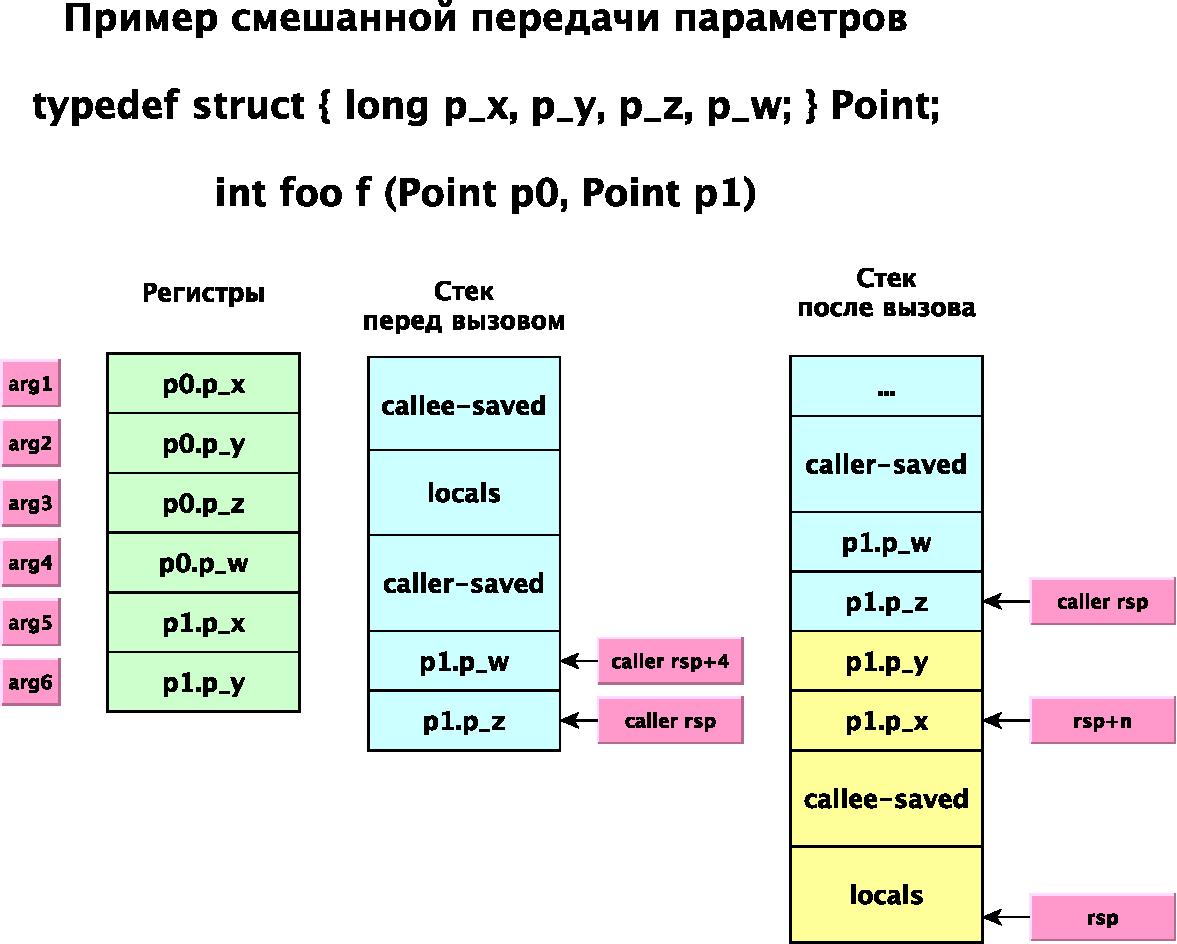
\includegraphics[width=1.0\textwidth]{illustrations/abi-sample-2-crop.pdf}
\caption{Пример передачи параметров}
\label{fig:abi}
\end{figure}

TODO: здесь какой-нибудь разбор этой картинки

Некоторые традиционные конвенции вызова имеют свои устоявшиеся имена:

\begin{itemize}
\item cdecl – через стек, справа налево, обратный сдвиг – caller 
\item pascal – через стек, слева направо, сдвиг – callee
\item fastcall – на регистрах, сдвиг – callee
\item stdcall – через стек, справа налево, сдвиг – callee
\item tailcall – вызов непосредственно перед возвратом, можно не двигать стек
\end{itemize}

\end{document}
